\documentclass[]{elsarticle} %review=doublespace preprint=single 5p=2 column
%%% Begin My package additions %%%%%%%%%%%%%%%%%%%
\usepackage[hyphens]{url}

  \journal{Applied Geography} % Sets Journal name


\usepackage{lineno} % add
\providecommand{\tightlist}{%
  \setlength{\itemsep}{0pt}\setlength{\parskip}{0pt}}

\usepackage{graphicx}
\usepackage{booktabs} % book-quality tables
%%%%%%%%%%%%%%%% end my additions to header

\usepackage[T1]{fontenc}
\usepackage{lmodern}
\usepackage{amssymb,amsmath}
\usepackage{ifxetex,ifluatex}
\usepackage{fixltx2e} % provides \textsubscript
% use upquote if available, for straight quotes in verbatim environments
\IfFileExists{upquote.sty}{\usepackage{upquote}}{}
\ifnum 0\ifxetex 1\fi\ifluatex 1\fi=0 % if pdftex
  \usepackage[utf8]{inputenc}
\else % if luatex or xelatex
  \usepackage{fontspec}
  \ifxetex
    \usepackage{xltxtra,xunicode}
  \fi
  \defaultfontfeatures{Mapping=tex-text,Scale=MatchLowercase}
  \newcommand{\euro}{€}
\fi
% use microtype if available
\IfFileExists{microtype.sty}{\usepackage{microtype}}{}
\bibliographystyle{elsarticle-harv}
\ifxetex
  \usepackage[setpagesize=false, % page size defined by xetex
              unicode=false, % unicode breaks when used with xetex
              xetex]{hyperref}
\else
  \usepackage[unicode=true]{hyperref}
\fi
\hypersetup{breaklinks=true,
            bookmarks=true,
            pdfauthor={},
            pdftitle={Patterns in Mongolian Nomadic Household Movement Derived from GPS Trajectories},
            colorlinks=false,
            urlcolor=blue,
            linkcolor=magenta,
            pdfborder={0 0 0}}
\urlstyle{same}  % don't use monospace font for urls

\setcounter{secnumdepth}{5}
% Pandoc toggle for numbering sections (defaults to be off)

\newlength{\cslhangindent}
\setlength{\cslhangindent}{1.5em}
\newenvironment{cslreferences}%
  {\setlength{\parindent}{0pt}%
  \everypar{\setlength{\hangindent}{\cslhangindent}}\ignorespaces}%
  {\par}

% Pandoc header
\usepackage{booktabs}
\usepackage{longtable}
\usepackage{array}
\usepackage{multirow}
\usepackage{wrapfig}
\usepackage{float}
\usepackage{colortbl}
\usepackage{pdflscape}
\usepackage{tabu}
\usepackage{threeparttable}
\usepackage{threeparttablex}
\usepackage[normalem]{ulem}
\usepackage{makecell}
\usepackage{xcolor}



\begin{document}
\begin{frontmatter}

  \title{Patterns in Mongolian Nomadic Household Movement Derived from
GPS Trajectories}
    \author[ifgi]{Henning Teickner}
   \ead{henning.teickner@uni-muenster.de} 
    \author[ifgi]{Christian Knoth\corref{1}}
   \ead{christian.knoth@uni-muenster.de} 
    \author[ifgi]{Thomas Bartoschek}
  
    \author[picir]{Kati Kraehnert}
  
    \author[feba]{Melinda Vigh}
  
    \author[dgnum]{Myagmartseren Purevtseren}
  
    \author[dgnum]{Munkhnaran Sugar}
  
    \author[ifgi]{Edzer Pebesma}
  
      \address[ifgi]{Institute for Geoinformatics, University of
Münster, Heisenbergstraße 2, DE-48149}
    \address[picir]{Potsdam Institute for Climate Impact Research}
    \address[feba]{Faculty of Economics and Business Administration,
Vrije Universiteit Amsterdam}
    \address[dgnum]{Department of Geography, National University of
Mongolia}
      \cortext[1]{Corresponding Author}
  
  \begin{abstract}
  This paper presents an approach for a quantitative analysis of
  movement patterns of nomadic households based on GPS trajectories. We
  distributed GPS loggers to 400 Mongolian herder households who carried
  them over a 9-month period, continuously recording position data every
  30 minutes. A total of 142 of the resulting trajectories fulfilled our
  data quality criteria and were considered during the analysis. Based
  on this data, we derive summary indicators describing key parameters
  of the households' mobility including measures of distance and number
  of movements as well as shape characteristics of the trajectories. We
  conduct an explorative statistical analysis of these summary
  indicators to investigate patterns in the nomadic mobility. We
  identify three movement strategies based on the number of different
  campsite locations and the distances traveled between campsites. We
  also compare the results to the existing literature on the mobility of
  Mongolian herders. Our findings show that GPS-based studies present a
  suitable framework to quantitatively analyze different movement
  strategies of nomadic herders.
  \end{abstract}
  
 \end{frontmatter}

\hypertarget{introduction}{%
\section{Introduction}\label{introduction}}

In Mongolia, which is among the five most heavily grazed countries in
the world (Sankey et al., 2012), mobile pastoralism is of great societal
importance, both economically and culturally. Mongolian grasslands form
the world's largest contiguous grazing area (Upton, 2005). On much of
this grassland, soil productivity is low and forage availability is
highly variable and difficult to predict. In this environment, permanent
agriculture and sedentary animal husbandry are rare whereas nomadic
herding is the predominant form of livelihood (Himmelsbach, 2012). In
2015, 25.2 percent of Mongolian households derived their livelihood
solely from herding (National Statistics Office of Mongolia, 2019). It
is the main economic activity in rural Mongolia, and the nomadic
lifestyle of Mongolian herders sustains this industry (Sankey et al.,
2012). Besides the economic aspects, nomadism carries immense cultural
value as a core element of Mongolian identity (Upton, 2010).

Climate change has an increasing impact on the livelihood of herders.
They are particularly affected by natural hazards and adverse climate
conditions because of the nature of their economic activities as well as
their geographic location (Intergovernmental Panel on Climate Change,
2014; World Bank, 2009). In Mongolia, the greatest environmental risk to
herding households is the growing frequency and severity of droughts and
events of extreme winter conditions, so called dzuds. These
catastrophes, which have occurred multiple times in recent years, lead
to mass livestock deaths and pose a significant threat of poverty and
forced outmigration of herding households to urban areas
(Lehmann-Uschner and Kraehnert, 2018; Sternberg, 2010). Since extreme
weather events are expected to become more frequent and intense as a
result of climate change (Intergovernmental Panel on Climate Change,
2013, 2007; Seneviratne et al., 2012), there is great need for concepts
to assist nomadic households in coping with these effects. This need is
increased by the fact that Mongolian rangelands are fragile and often
considered overused (Fernández-Giménez et al., 2018), and state
resources that can be invested in mitigation strategies are limited
(Stern, 2011).

In order to identify, understand and manage the specific negative
impacts of unfavorable climate conditions on herding households, a
better understanding of the mobility patterns of these households and
their movement strategies for adapting to environmental conditions is
crucial. Differences in mobility strategies (or the capacity to adopt
them) are a key factor influencing the capabilities of Mongolian herders
to cope with extreme weather events. In particular, the capability to
conduct movement over greater distances, and/or in shorter time spans
helps households to prevent high loss rates in the face of extreme
weather events (Murphy, 2011). As Fernández-Giménez et al. (2015) have
pointed out, mobility is a critical strategy not only during, but also
before and after dzud. Rapid movements of herds can be undertaken to
prepare for or escape a weather disaster (e.g.~drought or dzud)
(Fernández-Giménez et al., 2015).

To date, knowledge on the mobility patterns of Mongolian herders is
mainly based on household surveys and self-reported or estimated values
for quantitative parameters (Fernández-Giménez, 2006; Fernández-Giménez
et al., 2007, 1996). In such survey data, mobility information is
typically constrained by reporting bias and by the degree to which
respondents can reliably recall past movement retrospectively. In
contrast, nomadic migration profiles that are gathered using
anthropological field research methods are usually limited in their
representativeness. For example, Murphy (2011) bases his study of
nomadic households in Mongolia on a sample of four households that he
accompanied for several months. There is no study analyzing movement
patterns based on detailed geographic location data for a large number
of households. As a consequence, available information on nomadic
herders movement is mainly qualitative and restricted to a heuristic
classification of different movement types. Importantly, there has been
no attempt to analyze the interrelation of the frequency of movements,
the typical distance covered between subsequent campsite locations, and
the total distance covered in Mongolian nomadic movements.

An additional issue with existing literature is that most of the studies
date back to times during and even before the Soviet Union (Batnasan,
1978; Jagvaral, 1975; Simukov, 1934). Due to post-soviet changes in the
nomadic lifestyle and improved access to new transportation measures
(e.g.~trucks), it is unlikely that present movement of Mongolian nomads
is the same as at least 40 years ago (Fernández-Giménez, 2006; Marin,
2008). We found only one recent study (Ganbold, 2015) summarizing
Mongolian herders movement based on surveys with 50 households conducted
in 2003 to 2004.

In this paper we aim to demonstrate the value and feasibility of using
detailed movement data based on GPS measurements for deriving mobility
patterns of a large sample of nomadic households. We distributed GPS
loggers to 400 Mongolian herder households who carried them over a
9-month period. The loggers recorded the position measurements every 30
minutes, creating detailed household-level trajectories of the herders'
movements. Based on this data, we derived summary indicators describing
key parameters of the households' mobility patterns, such as the number
of movements to different campsites (and thereby pasture areas for the
herds), the distances and altitude differences covered between pasture
areas (in total and per movement), or the shape of the movement
trajectories. We describe the processing steps needed to derive
meaningful trajectories from the raw GPS data and for calculating the
summary indicators. We conduct an explorative statistical analysis of
these summary indicators and compare them to information on the mobility
of Mongolian herders from the existing literature.

In addition, we investigated whether there are distinct clusters of
households based on their movement characteristics, as suggested by
Jagvaral (1975). In previous research, the capability of herders to move
greater distances has been stated to be among the main factors affecting
their ability to cope with extreme weather conditions (see, e.g., Murphy
(2011)). Hence, we were interested in understanding if and how
households differ in terms of covering large distances as part of their
mobility strategies. Specifically, we investigated the relation between
(1) the total distance covered by households during the study period,
(2) the number of movements, and (3) the typical distance between
subsequent campsite locations. We hypothesize that the interrelation
between these characteristics is an important factor differentiating
their mobility practices. We performed a regression analysis to analyze
whether Mongolian households that move more often also cover larger
total distances and whether increasing the distance between subsequent
campsite locations may be a strategy to increase the total distance
covered. Moreover, the regression model enabled us to quantify to what
extent changes in both of these movement traits affect the total
distance covered.

To the best of our knowledge, this is the first time that GPS technology
is used for systematically studying detailed migration patterns of
nomadic families. Hence this paper is also meant to propose suggestions
for conducting such a study. We discuss the steps for collecting the GPS
data, practical risks and issues, economic considerations and lessons
learned during the study. In addition we elaborate on different aspects
of data quality and its implications for the analysis as well as the
applicability of the results for the prediction of climate impacts on
nomadic households and the development of coping strategies.

\hypertarget{methods}{%
\section{Methods}\label{methods}}

\hypertarget{study-area-and-collection-of-gps-data}{%
\subsection{Study Area and Collection of GPS
Data}\label{study-area-and-collection-of-gps-data}}

The collection of GPS data took place in Mongolia in 2015 and 2016. A
sub-sample of participating households was selected from the
\emph{Coping with Shocks in Mongolia Household Panel Survey} implemented
by the German Institute for Economic Research in collaboration with the
National Statistical Office of Mongolia (NSO). Given budget constraints
for purchasing GPS loggers and auxiliaries, the sample was restricted to
households in two survey provinces, Uvs and Zavkhan, with a total area
of 152,230 km\(^2\), which is about 10 \% of the area of the country.
Moreover, only those herding households were selected that reported
having moved their campsite at least once in the past 12 months in the
previous survey wave.

\begin{figure}[H]

{\centering 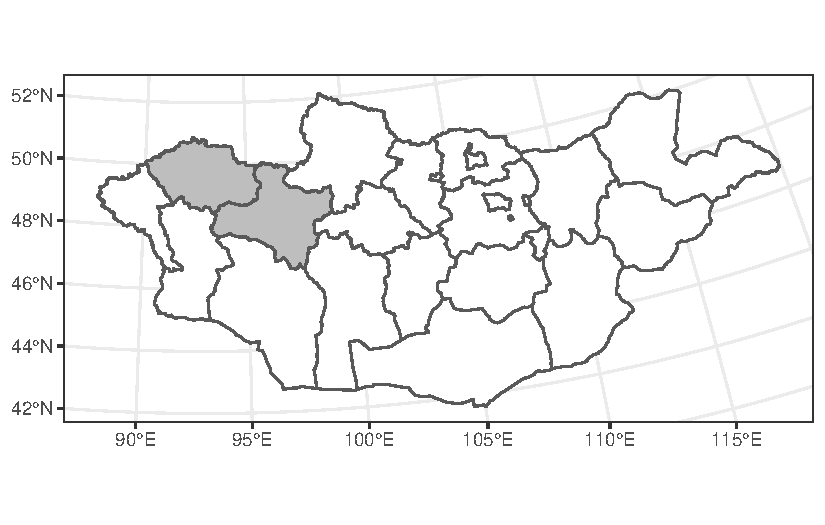
\includegraphics[width=0.8\textwidth]{../figures/aimags-map-1} 

}

\caption{Map of Mongolia with province boundaries. The two grey shaded provinces represent the study area (Uvs and Zavkhan, from west to east). In total, Mongolia has 22 provinces. Source: Administration Of Land Affairs, Geodesy And Cartography of Mongolia.}\label{fig:aimags-map}
\end{figure}

GPS loggers were handed over to 400 households during the first phase of
fieldwork in September and October 2015. During the second phase of
fieldwork, between June and July 2016, households were visited again.
GPS loggers were retrieved from 382 households, while 18 households
could not be located. Prior to fieldwork, we developed a detailed data
confidentiality protocol that follows the requirements of the German Act
on Data Confidentiality. Each household was asked for their written
consent to participate in the study. Households also received an
information sheet that explained the aims of the project and the data
protection measures.

The aim of the GPS data collection was to document nomadic movements
between campsites across seasons. Hence, the GPS loggers were attached
to the main pole in the middle of the ger, the movable tent used by
Mongolian nomads. Several measures were taken to maximize the GPS data
coverage during the study period. The GPS loggers were programmed with
an additional operating mode, which activated the devices only once
every 30 minutes. Applying this operating mode instead of continuously
recording allowed for up to three weeks of operating time per charge
cycle. Each household also received a small solar-powered battery
charger for recharging the logger. To reduce the dependency on weather
conditions and the risk of data loss due to battery outage, households
were additionally equipped with an external battery. This external
battery held enough capacity for multiple charges of the GPS logger and
could be recharged using the solar panel or other energy sources
whenever possible. Households were contacted regularly throughout the
study period via mobile phone, with a friendly reminder to recharge
batteries.

Each household received a monthly compensation of about
3\textasciitilde EUR, which was transferred via mobile phone credit. The
total costs for the equipment (GPS logger, SD card, solar-powered
battery charger, external battery) and compensation amounted to 146 EUR
per household.

\hypertarget{preprocessing-of-gps-data}{%
\subsection{Preprocessing of GPS Data}\label{preprocessing-of-gps-data}}

After collecting GPS loggers from households, the data were checked and
prepared for import and analysis. File corruptions causing import errors
(e.g., due to malfunctions during the file writing) were analyzed and -
whenever possible - corrected. Data analysis was conducted in the
open-source software environment R (R Core Team, 2017), using the
trajectories package (Pebesma et al., 2018) for handling the specific
trajectory data type and the herdersTA package (Teickner and Knoth,
2020) (release ``herdersmovementpatterns'') specifically developed for
this manuscript. The data was preprocessed to fit the requirements of
this study: Since some households accidentally operated the GPS loggers
in the continuous recording mode, all trajectories were downsampled to a
temporal resolution of 30 minutes to achieve the same sampling scheme
for all households. In light of the aim of this study, the subsequent
analysis does not consider intraday movements, but focuses only on
locations where households stayed overnight for a given amount of time.
Therefore, we considered only GPS data recorded during 00:00 AM and
04:00 AM. For short periods (up to four days) without recorded GPS
fixes, we assumed the overnight location of corresponding households as
being constant when the GPS fixes right before and after these periods
were no more than 800\textasciitilde meters apart. The threshold of 800
m was chosen based on visual inspection of the data, which revealed
considerable noise of the GPS signal (i.e., random positional changes
within a radius of a few hundred meters even during night time). We
assume that this noise originates from metal plates typically placed at
the top of the gers that disturbed the GPS readings. For this reason, a
large threshold had to be chosen to correctly assign individual GPS
records to the same location. A further reason was that upon multiple
visits of the same location, the ger was not always placed exactly at
the same position. Our experiments showed that a threshold of 800 m
assures that such visits are assigned to the same location and at the
same time preserves the separation between different neighboring
campsite locations.

\hypertarget{identification-of-campsite-locations-visits-and-movements}{%
\subsection{Identification of Campsite Locations, Visits and
Movements}\label{identification-of-campsite-locations-visits-and-movements}}

In the preprocessed data, campsite locations were then identified. This
was done using a two-step approach. First, we identified locations where
households remained stationary without major movement for a certain
amount of time. Here, density-based clustering (Hahsler and Piekenbrock,
2019) was applied to identify all locations with an accumulation of
fixes (minimum of six fixes within a radius of 800 meters). In a second
step, a household's presence at each of these locations was classified
as either short term visit or campsite, depending on the duration of the
stay. Only a continuous stay of four or more nights in a given location
was classified as a campsite visit of the corresponding household.
Inspection of those trajectories with very high data density (very few
gaps) revealed that short-term visits typically had a duration no longer
than four days. Due to the small amount of gaps in these cases and the
fact that after such visits the GPS logger returned to the previous
location with a longer visit, we assumed that these short-term visits
were distinct from long-term movements of the ger. Since a large
fraction of trajectories did not contain these short-term visits, but
larger gaps, we decided to consider a continuous visit of at least four
nights as campsite visit in contrast to a short-term visit.

To further increase data coverage with regards to campsite locations,
periods without location data were filled if they were shorter than 30
days and if the locations of a given household before and after the gap
was the same. In this case, we assumed that a household remained at the
same campsite. This was based on the assumption that when the nomadic
households move their campsites away from a certain location they do not
move it back to that location within less than 30 days. Finally, we
computed the median values of the original coordinates for each
identified campsite location. This was possible for 348 of the 400
households that had received GPS loggers. For the remaining households,
either the GPS loggers could not be recollected because the households
could not be located, GPS data was not recorded due to technical
failures, or no more than one campsite location could be identified
according to our criteria, which made it impossible to compute most of
the movement summary indicators.

\hypertarget{gap-filtering-and-temporal-constraints}{%
\subsection{Gap Filtering and Temporal
Constraints}\label{gap-filtering-and-temporal-constraints}}

While it is reasonable to fill periods without location data up to
certain durations in light of the item of our analysis (campsite
locations), longer periods cannot be filled without reducing confidence
in the data and were therefore considered gaps. Data gaps potentially
have important consequences for the analysis of movement patterns. Since
movements occur at distinct time periods and the duration of the visit
of a campsite location can vary (according to our definition) from four
days to any longer duration, it is possible that visits of campsite
locations are missed. This may lead to biased estimates of important
movement characteristics, for example the number of different campsite
locations visited or the covered distance, and consequently bears the
risk of misleading interpretations. An uneven distribution of the
proportion of gaps across households may represent another source of
information bias. Consequently, it is important to control for the
amount of gaps during the analysis of movement patterns. Additionally,
the maximum duration of any gap is an important factor because the
longer a gap is, the larger is the probability that a campsite visit was
not recorded. Therefore, the trajectories were filtered both according
to their proportion of gaps and the maximum duration of the gaps.
Filtering refers to removing households that do not meet certain
threshold values (for the proportion of gaps and the maximum duration of
the gaps) from the sample of households. Unfortunately, there exist no
best practices for setting thresholds for both variables. We used a
density plot in order to identify thresholds in the proportion of gaps
and the maximum duration of the gaps so that households with large
proportions of gaps and gaps with a large duration were excluded, but a
sample of sufficient size was retained (figure 2). A trade-off between
loosing too many observations and applying conservative thresholds of
acceptance was found by setting the maximum proportion of missing values
to 30 \% and the maximum duration of any gap to 30 days for the complete
study period (see next paragraph).

The time range of the GPS trajectories of different households varied.
Reasons for this are that (1) the GPS loggers could not be distributed
and recollected at the same time, (2) households differed in the way
they handled the GPS devices, which may have resulted in different
operating modes, and (3) gaps in the data also occur at the start and
the end of the trajectories. Because several of the movement summary
indicators we computed covary with the time, this varying temporal
coverage may lead to artifacts, for example a difference in the number
of visited campsite locations. To account for this, we clipped all data
to a common study period. Defining start and end points of this study
period is not a trivial problem because a trade-off between minimizing
gaps for some households and enlarging temporal coverage, and hence
representativeness, has to be found. We defined the starting point of
the study period as median of the time points where the first GPS fixes
were recorded (2015-10-01). The end of the study period was defined as
the median of the time points where the last GPS fixes were recorded
(2016-06-22, figure 3). Thus, the data cover a time period of 265 days
and comprise several campsite locations before and after the winter
campsite location, where households stay for a longer time period.

\begin{figure}[H]

{\centering 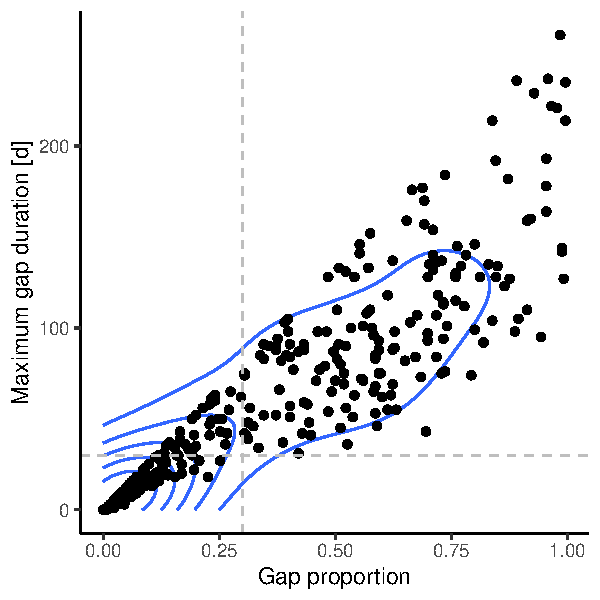
\includegraphics[width=0.7\textwidth]{../figures/gap-filtering-study-period-plot1-1} 

}

\caption{Density plot for the duration of the longest gap in the trajectory and the proportion of gaps (relative number of days without identified location during the study period) in the preprocessed trajectories computed for each of the 348 Mongolian nomadic households. The vertical dashed line represents the threshold value for the proportion of gaps (30\,\%) and the horizontal dashed line the threshold value for the duration of the longest gap (30 days). The blue lines are contour lines for the density of the data points. Note that the density of households below the threshold values indicated by the dashed lines is larger than that of the households not matching these thresholds.\label{fig:gap_filtering_study_period_plot1}}\label{fig:gap-filtering-study-period-plot1}
\end{figure}

\begin{figure}[H]

{\centering 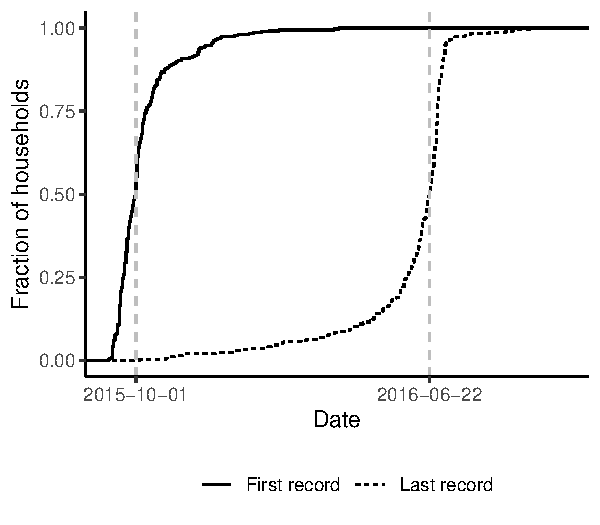
\includegraphics[width=0.7\textwidth]{../figures/gap-filtering-study-period-plot2-1} 

}

\caption{Cumulative densities for the day where the first location was recorded (first day of the first recorded location, solid line) and the day where the last location was recorded (last day of the last recorded location, dashed line), computed for the 348 Mongolian nomadic households. Vertical dashed lines represent the median value of the days where the first location was recorded and the days where the last location was recorded, respectively, and these values are defined as start and end time points of the study period, respectively. \label{fig:gap_filtering_study_period_plot2}}\label{fig:gap-filtering-study-period-plot2}
\end{figure}

\hypertarget{computation-of-movement-summary-indicators}{%
\subsection{Computation of Movement Summary
Indicators}\label{computation-of-movement-summary-indicators}}

For each household, we computed the movement summary indicators defined
and described in table 1 based on the trajectories of identified
campsite locations. The aim was to define a set of movement summary
indicators that represent the horizontal and vertical movements,
trajectory shape (movement direction, movement direction change,
straightness index), inter-campsite location distances, number of
campsite locations and visits, and the spatial range covered.

The definition of the straightness index (Laube et al., 2007) is
visualized conceptually in figure 7. It is computed by (1) calculating
the sum of the lengths of the individual inter-campsite beeline
distances along the trajectory (length of the trajectory) \(a\), (2)
calculating the beeline distance between the first and last campsite
location of the trajectory, \(b\), and (3) dividing \(a\) by \(b\)
(Laube et al., 2007).

The derivation of the trajectory linearity is visualized in figure 8. In
order to calculate one value, at least three campsite locations have to
be present in a trajectory. The trajectory linearity is computed by (1)
computing all pairwise distances between all campsite locations in the
trajectory, (2) retaining the maximum distance \(a\) and constructing a
line \(line_a\) between the corresponding two campsite locations, (3)
computing the shortest distance between each campsite locations and
\(line_a\) and (4) recording on which side of the line the campsite
locations are placed. (5) If there are only campsite locations on one
side of the line, the maximum distance between a campsite location and
\(line_a\) is recorded as \(b\), else the maximum sum of the distances
of two campsite locations on different sides of the line to \(line_a\)
(\(b_1\) and \(b_2\)) is recorded as \(b = b_1 + b_2\), and (6) finally,
the trajectory linearity is computed as \(a/b\).

\begingroup\fontsize{7}{9}\selectfont

\begin{longtable}[t]{llp{23em}}
\caption{\label{tab:movement-summary-indicators-definition}Definition of the movement summary indicators. \label{tab:movement_summary_indicators_definition}}\\
\toprule
ID & Summary Indicator & Definition\\
\midrule
1 & location\_altitude\_difference & The altitude difference between the two campsite locations with the extreme altitude values (minimum, maximum) in a trajectory [m].\\
2 & total\_altitude\_distance & The sum of the absolute altitude differences (beeline distances) covered along the trajectory, i.e. between following campsite locations [m].\\
3 & location\_distance & The median distance between following campsite locations [m].\\
4 & total\_distance & The total distance covered by a household [m].\\
5 & longitude\_difference & The absolute longitude difference between the two campsite locations with the extreme longitude values (minimum, maximum) in a trajectory [m].\\
\addlinespace
6 & latitude\_difference & The absolute latitude difference between the two campsite locations with the extreme longitude values (minimum, maximum) in a trajectory [m].\\
7 & longitude\_sum & The absolute longitude difference between the first and last campsite location in a trajectory [m].\\
8 & latitude\_sum & The absolute latitude difference between the first and last campsite location in a trajectory [m].\\
9 & chull\_area & The area of a convex hull spanned around all campsite locations of a trajectory [m$^2$].\\
10 & chull\_perimeter & The perimeter of a convex hull spanned around all campsite locations of a trajectory [m].\\
\addlinespace
11 & linearity & An estimate of the trajectory linearity. See figure~8 for a conceptual graphic and the text for more details.\\
12 & straightness\_index & The ratio of total\_distance and the beeline distance between the first and last campsite location in a trajectory (Laube et al., 2007). See figure 7.\\
13 & locations\_number & The number of different campsite locations along a trajectory.\\
14 & locations\_number\_repeated\_visits & The number of repeated visits of all campsite locations along a trajectory.\\
\bottomrule
\end{longtable}
\endgroup{}

\hypertarget{statistical-analysis}{%
\subsection{Statistical Analysis}\label{statistical-analysis}}

We conducted an explorative analysis to characterize overall patterns in
the computed movement summary indicators. Based on this, we tested for
distinct clusters of households based on these indicators. Finally, we
investigated in more detail the relation between the total distance
moved, the number of visited campsite locations, and the median distance
between subsequent campsite locations. We created scatterplots and
computed a linear regression model that allowed us to quantify how
changes in the number of visited campsite locations and the median
distance between subsequent campsite locations influence the total
distance covered. All computations were conducted in the programming
language R (R Core Team, 2017) and all plots (except stated differently)
were created using the R packages ggplot2 (Wickham, 2016) and cowplot
(Wilke, 2018).

\hypertarget{summary-table}{%
\subsubsection{Summary Table}\label{summary-table}}

First, we summarized the summary indicators described above by computing
their mean, median, minimum, and maximum values. This summary is
provided in table 2 to give a detailed overview on typical ranges of the
summary indicators for Mongolian nomadic household movements. Note that
for the linearity indicator, only households with \(\ge 3\) campsite
locations were considered. We also summarized the proportion of gaps in
the samples in this table.

\hypertarget{correlation-analysis}{%
\subsubsection{Correlation Analysis}\label{correlation-analysis}}

Second, we computed the Pearson correlation between the movement summary
indicators in order to analyze their pairwise relation. Samples with
\(< 3\) campsite locations were excluded. Otherwise, it would not have
been possible to include the trajectory linearity as variable in the
analysis. Summary indicators with highly skewed sample densities were
log-transformed prior the analysis (chull\_area, chull\_perimeter,
location\_altitude\_difference, location\_distance,
longitude\_difference, latitude\_diffe-rence, straightness\_index,
total\_altitude\_distance, total\_distance and linearity; see figure
10).

\hypertarget{principal-component-analysis}{%
\subsubsection{Principal Component
Analysis}\label{principal-component-analysis}}

Third, we conducted a principal component analysis (PCA) on the movement
summary indicators in order to analyze main gradients formed by the
households and the multivariate relation between the computed movement
summary indicators. For this, the same data as used for the correlation
analysis (log-transformation of skewed variables, only households that
visited \(\ge 3\) campsite locations), but excluding the number of
campsite locations, was used. In addition, all summary indicators were
z-transformed prior computing the PCA. We applied the Kaiser-Guttman
criterion (Jackson, 1993) to select the first \(n\) principal components
(PCs) for interpretation. PCs were interpreted by computing the relative
importance of each summary indicator variable for the PC, the loadings
of the summary indicator variables for the PCs and by creating biplots
of the loadings for different combinations of retained PCs. The loading
values of a variable represent how this variable relates to a PC.
Positive loadings of a variable for a PC indicate that positive values
of the variable increase the score value of a sample for this PC.
Gradients along the PCs and potential clustering were assessed by
creating biplots of the scores of the PCA for different combinations of
retained PCs. The PCA was computed using the R package vegan (Oksanen et
al., 2018).

\hypertarget{hierarchical-cluster-analysis}{%
\subsubsection{Hierarchical Cluster
Analysis}\label{hierarchical-cluster-analysis}}

Third, we computed a hierarchical cluster analysis with the aim to
identify distinct groups of households with the same movement
characteristics. For this, we used a subset of the movement summary
indicators presented above because both the PCA and correlation analysis
revealed that several movement summary indicators are correlated and
probably indicate similar underlying factors. Besides, we used the same
observations as included in the PCA, meaning that only households with
at least 3 campsite locations were included in the cluster analysis. All
included variables were z-transformed prior the analysis to give all
variables equal weights. We did not log-transform skewed variables to
preserve differences at their original scale. The Euclidean distance was
used as distance measure.

Different hierarchical clustering algorithms exist. Ward's minimum
variance clustering (WMVC) is widely used and seeks to partition the
data such that the within cluster sum of squared distances are minimized
(Borcard et al., 2011). Single linkage clustering (SLC) agglomerates
groups based on pairwise distances between objects within the clusters.
If the pairwise distance between two objects in different clusters with
the least distance to each other is the least among different groups,
the two groups are merged. This facilitates so-called chaining where
individual observations are linked sequentially, thus representing
gradients more appropriately (Borcard et al., 2011). Complete linkage
clustering (CLC) works in the same way as single linkage clustering, but
two objects are merged into one cluster if the pairwise distance between
two objects in different clusters with the maximum distance to each
other is the least among different groups. The consequence is that
multiple small groups are formed with more spherical shape in the
multivariate space, i.e.~(small-scale) discontinuities are pronounced by
CLC (Borcard et al., 2011).

Each clustering algorithm results in a dendrogram representing the
relative distances between samples and the stepwise partitioning of the
data, where at each step the number of clusters is increased. Clustering
representativeness for each cluster method was assessed by (1) computing
the Pearson correlation between the sample Euclidean distances and the
cophenetic distances of the clustering results (cophenetic correlation)
and (2) computing average silhouette widths for selected cluster subsets
of the computed dendrograms (Borcard et al., 2011). The larger the
cophenetic correlation between the cophenetic distances of a dendrogram
and the sample Euclidean distances, the larger is the ability of a
dendrogram to represent patterns in the data (Borcard et al., 2011). The
larger average silhouette width for selected cluster subsets of the
computed dendrograms the larger is the similarity of samples within each
cluster (Borcard et al., 2011). A subset of the clusters provided by
each dendrogram was identified by applying partition around medoids
(PAM) on the cophenetic distance matrices such that the average
silhouette width was maximized (Maechler et al., 2018). Thus, computing
average silhouette widths also yielded estimates of the number of
clusters to interpret (Maechler et al., 2018). Since the cluster results
indicated that a gradual description of the movement summary indicators
across the sampled households is more appropriate (see section
\protect\hyperlink{hierarchical-cluster-analysis-1}{3.5}), we did not
interpret the identified clusters. Clusters and dendrograms were
computed using functions of the R packages stats (R Core Team, 2017),
cluster (Maechler et al., 2018) and dendextend (Galili, 2015).

\hypertarget{regression-analysis}{%
\subsubsection{Regression Analysis}\label{regression-analysis}}

Since the PCA and hierarchical cluster analysis did not identify a
clustered structure of the movement summary indicator data, we used a
regression model and scatterplots to describe in more detail the
relations between our two target movement summary indicators (the number
of visited campsite locations and the median distance between subsequent
campsite locations) and the total distance covered. The aim was to
identify movement strategies across this gradient and to provide
evidence for our hypothesis that different mobility practices of the
nomadic herder households are differentiated by the interrelations
between these characteristics.

The mobility range, as indicated by the total distance covered, is
potentially an important variable for forage and water availability and
avoidance of unfavorable climate conditions. Theoretically, it is
possible for a household to increase the total distance covered by (1)
visiting more campsite locations along the way and (2) increasing the
distance of individual movements between subsequent campsite locations.
Both strategies may be applied simultaneously. Making long-distance
movements between subsequent campsite locations in comparison to making
movements with smaller distances but higher frequency (i.e.~having more
campsite locations) potentially has implications for the resources spent
on movements, the risk of movements, and may be a result of differences
in herd size and availability of resources (Marin, 2008). The median
distance of individual movements between subsequent campsite locations
(location\_distance) is an indicator for both an increase in the
distance of individual movements and an increase \emph{in the frequency}
of movements with at least such a distance.

For the regression analysis, we used a generalized linear regression
model (GLM) with Gamma distribution to account for the fact that the
total distance covered cannot be negative. Both the number of visited
campsite locations and the median distance between subsequent campsite
locations were log transformed prior the analysis since this reduced
non-linear patterns in the residuals. We computed the regression model
in R (R Core Team, 2017), the variance explained following Nakagawa et
al. (2017) using the package MuMIn (Barton, 2020), confidence intervals
using the package MASS (Venables and Ripley, 2007) and validated the
models with residual plots and plots of predicted values using the
packages ggplot2 (Wickham, 2016), cowplot (Wilke, 2018), and
directlabels (Hocking, 2020).

\hypertarget{results}{%
\section{Results}\label{results}}

\hypertarget{gps-data-quality}{%
\subsection{GPS Data Quality}\label{gps-data-quality}}

The 348 households for which campsite locations could be detected
(i.e.~prior gap filtering) had an average proportion of gaps of 34 \%
(median = 25 \%) with a minimum of 0 \% and a maximum of 100 \% after
gap filling. The duration of a gap per household was on average 34 days
(median = 25, minimum = 0 days, maximum = 261 days). The number of gaps
per household ranged from 1 to 12 and the median was 2. 147 households
fulfilled our data quality criteria and were used in the explorative
analysis. For these households, no clear relation between the value of
any movement summary indicator and the proportion of gaps was visible,
indicating that after filtering, the sample likely is unbiased regarding
the values of the summary indicators (figure 9). Note that for the
correlation analysis, PCA, and cluster analysis we further restricted
this sample to the households with \(\ge 3\) campsite locations (n =
142) because the trajectory linearity could not be computed for
households with less than three visited campsite locations.

\hypertarget{movement-summary-indicators}{%
\subsection{Movement Summary
Indicators}\label{movement-summary-indicators}}

In table 2, we present summary statistics for the computed movement
summary indicators for the sampled households. Total beeline movement
distances between campsite locations ranged from 7 to 364.8 km, median
distances between adjacent campsite locations between 2.3 and 125.8 km
and the number of campsite locations from 2 to 14. Using a threshold
value of 4 days to differentiate between campsite visits and short-term
visits, 0 to 18 short-term visits were recorded (median = 1, n = 147)
for the households. There were 0 to 18 locations per household for which
only short-term visits were recorded (median = 0, n = 147). Several
households had up to 3 repeated campsite visits at campsite locations.

\begingroup\fontsize{7}{9}\selectfont

\begin{longtable}[t]{lrrrrr}
\caption{\label{tab:results-summary-indicator-table}Overview of the values of the movement summary indicators and the proportion of days without data values (gaps\_proportion) for the household sample (gap filled with a threshold of 30 days and filtered with a maximum duration of any gap $\le 30$~days). Horizontal distances are given in km, chull\_area in km$^2$ and altitudinal distances in m. \label{tab:si_overview}}\\
\toprule
Summary Indicator & Mean & Median & Min & Max & n\\
\midrule
location\_altitude\_difference & 425.39 & 304.00 & 6.00 & 1445.00 & 147\\
total\_altitude\_distance & 1053.32 & 644.00 & 12.00 & 5222.00 & 147\\
location\_distance & 12.38 & 9.59 & 2.33 & 125.79 & 147\\
total\_distance & 78.44 & 60.83 & 7.04 & 364.84 & 147\\
longitude\_difference & 21.10 & 15.41 & 0.35 & 125.61 & 147\\
\addlinespace
latitude\_difference & 31.75 & 23.63 & 2.37 & 155.80 & 147\\
longitude\_sum & 1.37 & 0.75 & -31.72 & 66.80 & 147\\
latitude\_sum & 3.80 & 1.28 & -56.00 & 69.93 & 147\\
chull\_area & 320.10 & 98.15 & 0.00 & 4793.85 & 147\\
chull\_perimeter & 84207.29 & 64819.41 & 8734.26 & 368280.61 & 147\\
\addlinespace
locations\_number & 5.53 & 5.00 & 2.00 & 14.00 & 147\\
locations\_number\_repeated\_visits & 0.57 & 0.00 & 0.00 & 3.00 & 147\\
straightness\_index & 6.80 & 3.35 & 1.00 & 112.21 & 147\\
linearity & 7.61 & 4.53 & 1.12 & 68.31 & 142\\
gaps\_proportion & 0.05 & 0.04 & 0.00 & 0.25 & 147\\
\bottomrule
\end{longtable}
\endgroup{}

\hypertarget{correlation-analysis-1}{%
\subsection{Correlation Analysis}\label{correlation-analysis-1}}

All Pearson correlation coefficients are presented in table 3. Many
variables are positively related to the total distance covered: the
largest pairwise longitudinal and latitudinal distance between campsite
locations, the area and perimeter of a convex hull for the campsite
locations, the total altitudinal distance covered and also the number of
visited locations and median distance between subsequent campsite
locations. This indicates that these variables are all indicators of
increased mobility in general. Linearity and straightness index were not
strongly related to any other movement summary indicator. The number of
visited locations was not related to the median distance between
subsequent campsite locations (table 3).

\begin{landscape}\begingroup\fontsize{8}{10}\selectfont

\begin{longtable}[t]{llllllllllllll}
\caption{\label{tab:results-correlation-analysis-table}Pearson correlation coefficients for all pairwise comparisons of the computed movement summary indicators for the 142 Mongolian nomadic households with at least 3 campsite locations. Absolute values $\ge 0.6$ are given in bold to facilitate visual interpretation. \label{tab:si_correlation}}\\
\toprule
\rotatebox{-90}{ } & \rotatebox{-90}{location\_altitude\_difference} & \rotatebox{-90}{total\_altitude\_distance} & \rotatebox{-90}{location\_distance} & \rotatebox{-90}{total\_distance} & \rotatebox{-90}{longitude\_difference} & \rotatebox{-90}{latitude\_difference} & \rotatebox{-90}{longitude\_sum} & \rotatebox{-90}{latitude\_sum} & \rotatebox{-90}{chull\_area} & \rotatebox{-90}{chull\_perimeter} & \rotatebox{-90}{linearity} & \rotatebox{-90}{straightness\_index} & \rotatebox{-90}{locations\_number}\\
\midrule
location\_altitude\_difference & \textbf{1} & \textbf{0.95} & 0.38 & 0.57 & 0.39 & 0.51 & 0.17 & 0.31 & 0.53 & 0.52 & -0.04 & 0.28 & 0.47\\
total\_altitude\_distance & \textbf{0.95} & \textbf{1} & 0.41 & \textbf{0.7} & 0.49 & 0.59 & 0.17 & 0.31 & \textbf{0.65} & \textbf{0.62} & -0.04 & 0.38 & 0.59\\
location\_distance & 0.38 & 0.41 & \textbf{1} & \textbf{0.65} & 0.52 & 0.55 & 0.04 & 0.13 & 0.55 & \textbf{0.64} & 0.31 & 0.35 & 0.1\\
total\_distance & 0.57 & \textbf{0.7} & \textbf{0.65} & \textbf{1} & \textbf{0.75} & \textbf{0.87} & 0.09 & 0.29 & \textbf{0.91} & \textbf{0.96} & 0.23 & 0.37 & \textbf{0.68}\\
longitude\_difference & 0.39 & 0.49 & 0.52 & \textbf{0.75} & \textbf{1} & 0.48 & 0.13 & 0.18 & \textbf{0.82} & \textbf{0.76} & 0 & 0.28 & 0.46\\
\addlinespace
latitude\_difference & 0.51 & 0.59 & 0.55 & \textbf{0.87} & 0.48 & \textbf{1} & 0.1 & 0.36 & \textbf{0.8} & \textbf{0.9} & 0.32 & 0.14 & \textbf{0.61}\\
longitude\_sum & 0.17 & 0.17 & 0.04 & 0.09 & 0.13 & 0.1 & \textbf{1} & 0.28 & 0.07 & 0.11 & 0.05 & 0.06 & 0.15\\
latitude\_sum & 0.31 & 0.31 & 0.13 & 0.29 & 0.18 & 0.36 & 0.28 & \textbf{1} & 0.32 & 0.35 & 0.07 & -0.06 & 0.28\\
chull\_area & 0.53 & \textbf{0.65} & 0.55 & \textbf{0.91} & \textbf{0.82} & \textbf{0.8} & 0.07 & 0.32 & \textbf{1} & \textbf{0.92} & -0.04 & 0.21 & \textbf{0.66}\\
chull\_perimeter & 0.52 & \textbf{0.62} & \textbf{0.64} & \textbf{0.96} & \textbf{0.76} & \textbf{0.9} & 0.11 & 0.35 & \textbf{0.92} & \textbf{1} & 0.3 & 0.22 & \textbf{0.63}\\
\addlinespace
linearity & -0.04 & -0.04 & 0.31 & 0.23 & 0 & 0.32 & 0.05 & 0.07 & -0.04 & 0.3 & \textbf{1} & 0.1 & -0.09\\
straightness\_index & 0.28 & 0.38 & 0.35 & 0.37 & 0.28 & 0.14 & 0.06 & -0.06 & 0.21 & 0.22 & 0.1 & \textbf{1} & 0.25\\
locations\_number & 0.47 & 0.59 & 0.1 & \textbf{0.68} & 0.46 & \textbf{0.61} & 0.15 & 0.28 & \textbf{0.66} & \textbf{0.63} & -0.09 & 0.25 & \textbf{1}\\
gaps\_proportion & -0.05 & -0.1 & 0.11 & -0.12 & -0.08 & -0.03 & -0.1 & -0.08 & -0.08 & -0.08 & 0.01 & 0.07 & -0.27\\
\bottomrule
\end{longtable}
\endgroup{}
\end{landscape}

\hypertarget{principal-component-analysis-1}{%
\subsection{Principal Component
Analysis}\label{principal-component-analysis-1}}

The first 4 PCs were selected according to the Kaiser-Guttman criterion
for further interpretation. They explain 49.9, 11.4, 10.3 and 9 \% of
the variance, respectively.

The first PC was related to the total distance the households covered,
as indicated by the biplots (figure 4), the relative variable
contribution of the total distance covered to the first PC and the
corresponding loading value. In addition, biplots, relative variable
contributions and loading values also indicate that several of the
movement summary indicators are strongly related to the total distance
covered (figure 4), in accordance with the correlation analysis (table
3). No variable had positive loadings for the first PC (figure 4).

The second PC was mainly related to the trajectory linearity, altitude
distance covered and altitude difference between the lowest and highest
campsite location, with households with more linear trajectory covering
smaller altitudinal distances and having a smaller maximum altitude
distance between campsite locations. However, a scatterplot of both
variables did not indicate a negative correlation, but a large variance.

The third PC had largest relative contributions from the net
longitudinal and latitudinal movement between the start and end of the
study period (figure 4), differentiating households that had a net
movement to the north and east from households that had a net movement
to the south and west. The straightness index is negatively related to
the net longitudinal and latitudinal movement. A biplot of the first and
third PC indicated that the net longitudinal and latitudinal movement
were related (Pearson correlation coefficient of log-transformed and
z-transformed variables = 0.28).

The fourth PC represented a gradient of trajectory linearity and
straightness index differentiating households with more linear
trajectory and larger straightness index from households with less
linear trajectory and straightness index.

The biplots of the scores revealed no clear clustering patterns, except
for the combinations of the first and third PC (figure 4). For these two
PCs, the biplot shows two clusters that are more differentiated for
negative values of PC1 (households covering larger distances) than for
positive values (where the clusters overlap at their extremes).

\begin{figure}[H]

{\centering 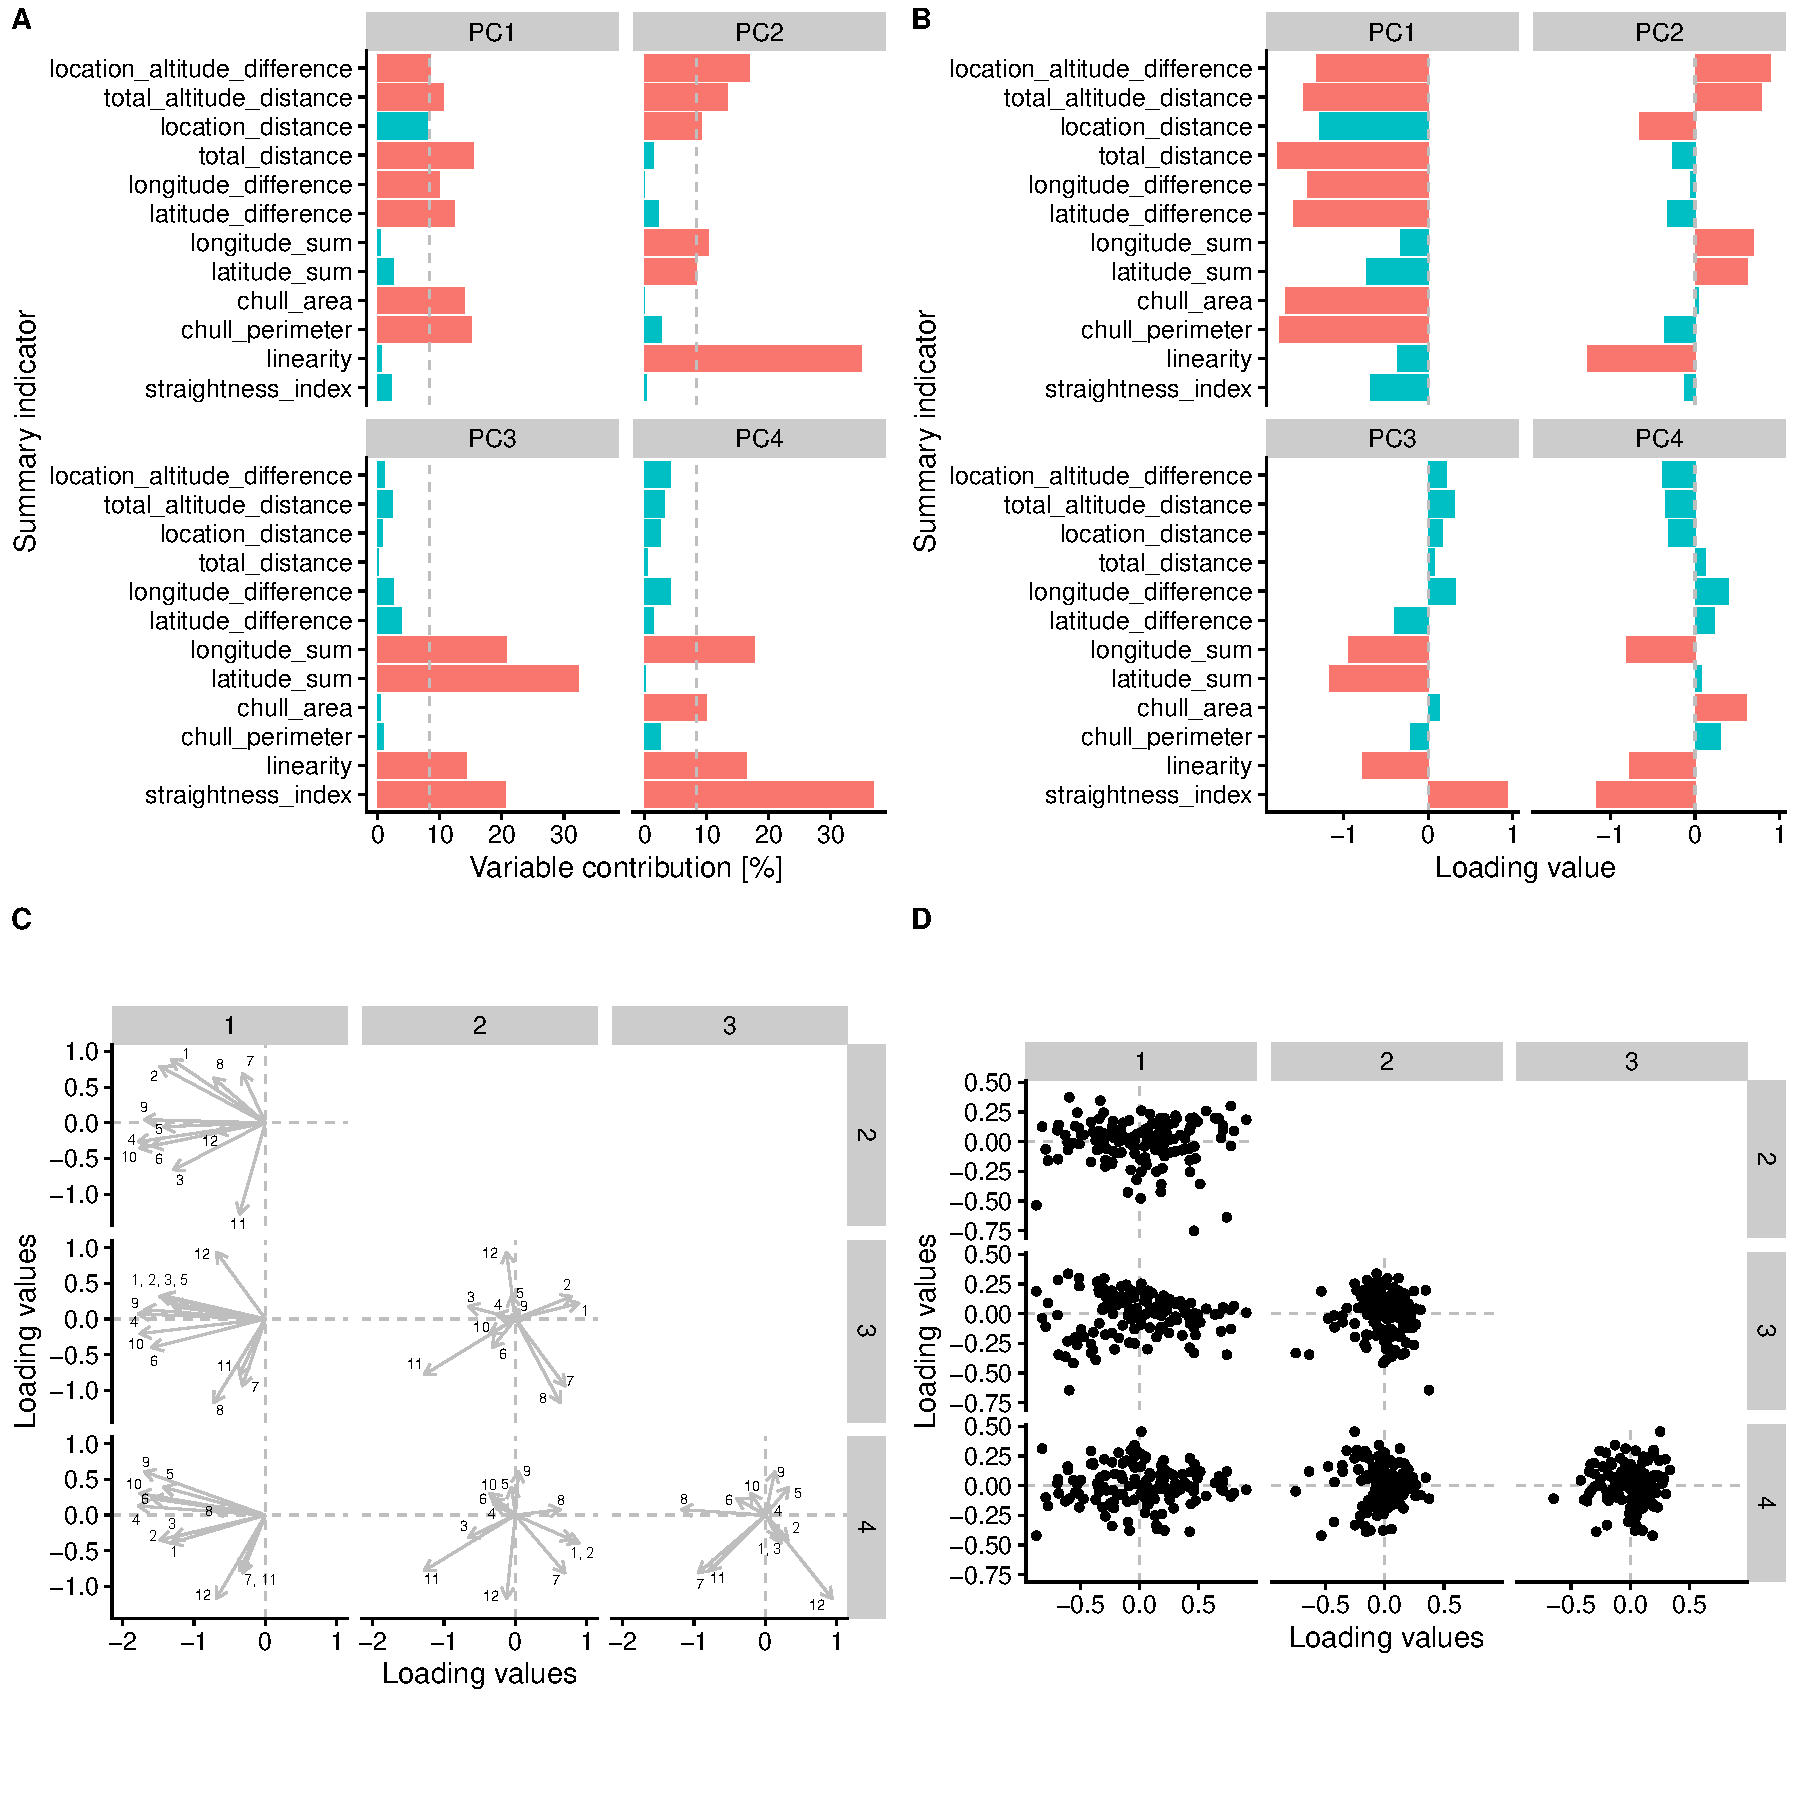
\includegraphics[width=\textwidth]{./../figures/si_pca_plots_derived} 

}

\caption{Plots for the principal component analysis (PCA) of the movement summary indicators computed for 142 Mongolian nomadic households with at least 3 campsite locations. A: Relative variable contribution [\%] for the first 4 PCs and each included variable. The dashed vertical line represents the average relative variable contribution in each case. Summary indicators contributing more than average to a PC have red filled bars. B: Plot of the loadings for the first 4 PCs. Summary indicators contributing more than average to a PC have red filled bars. C: Biplot of the loadings for all combinations of the first 4 PCs. Numbers refer to movement summary indicator IDs given in table 1. D: Biplot of the scores for all combinations of the first 4 PCs.}\label{fig:si-pca-plots-preparation}
\end{figure}

\hypertarget{hierarchical-cluster-analysis-1}{%
\subsection{Hierarchical Cluster
Analysis}\label{hierarchical-cluster-analysis-1}}

Cophenetic correlations of 0.68, 0.91 and 0.9 for WMVC, SLC and CLC,
respectively, indicated that SLC represents the original distance matrix
best (figure 5). The PAM-derived average silhouette widths derived from
PAM applied on the cophenetic distances also indicated that the SLC
maximizes the within cluster similarity: The average silhouette widths
were 0.64, 0.93 and 0.55 for the WMVC, SLC and CLC, respectively. For
SLC, the dendrogram showed chaining effects (figure 5). The number of
clusters maximizing the average silhouette width was 11, 2 and 2 for the
WMVC, SLC and CLC, respectively, with ranges of cluster sizes of 1 to
27, 1 to 141 and 16 to 126. Altogether, these results indicate that the
sampled households represent a gradient of the movement summary
indicators and do not form distinct groups.

\begin{figure}[H]

{\centering 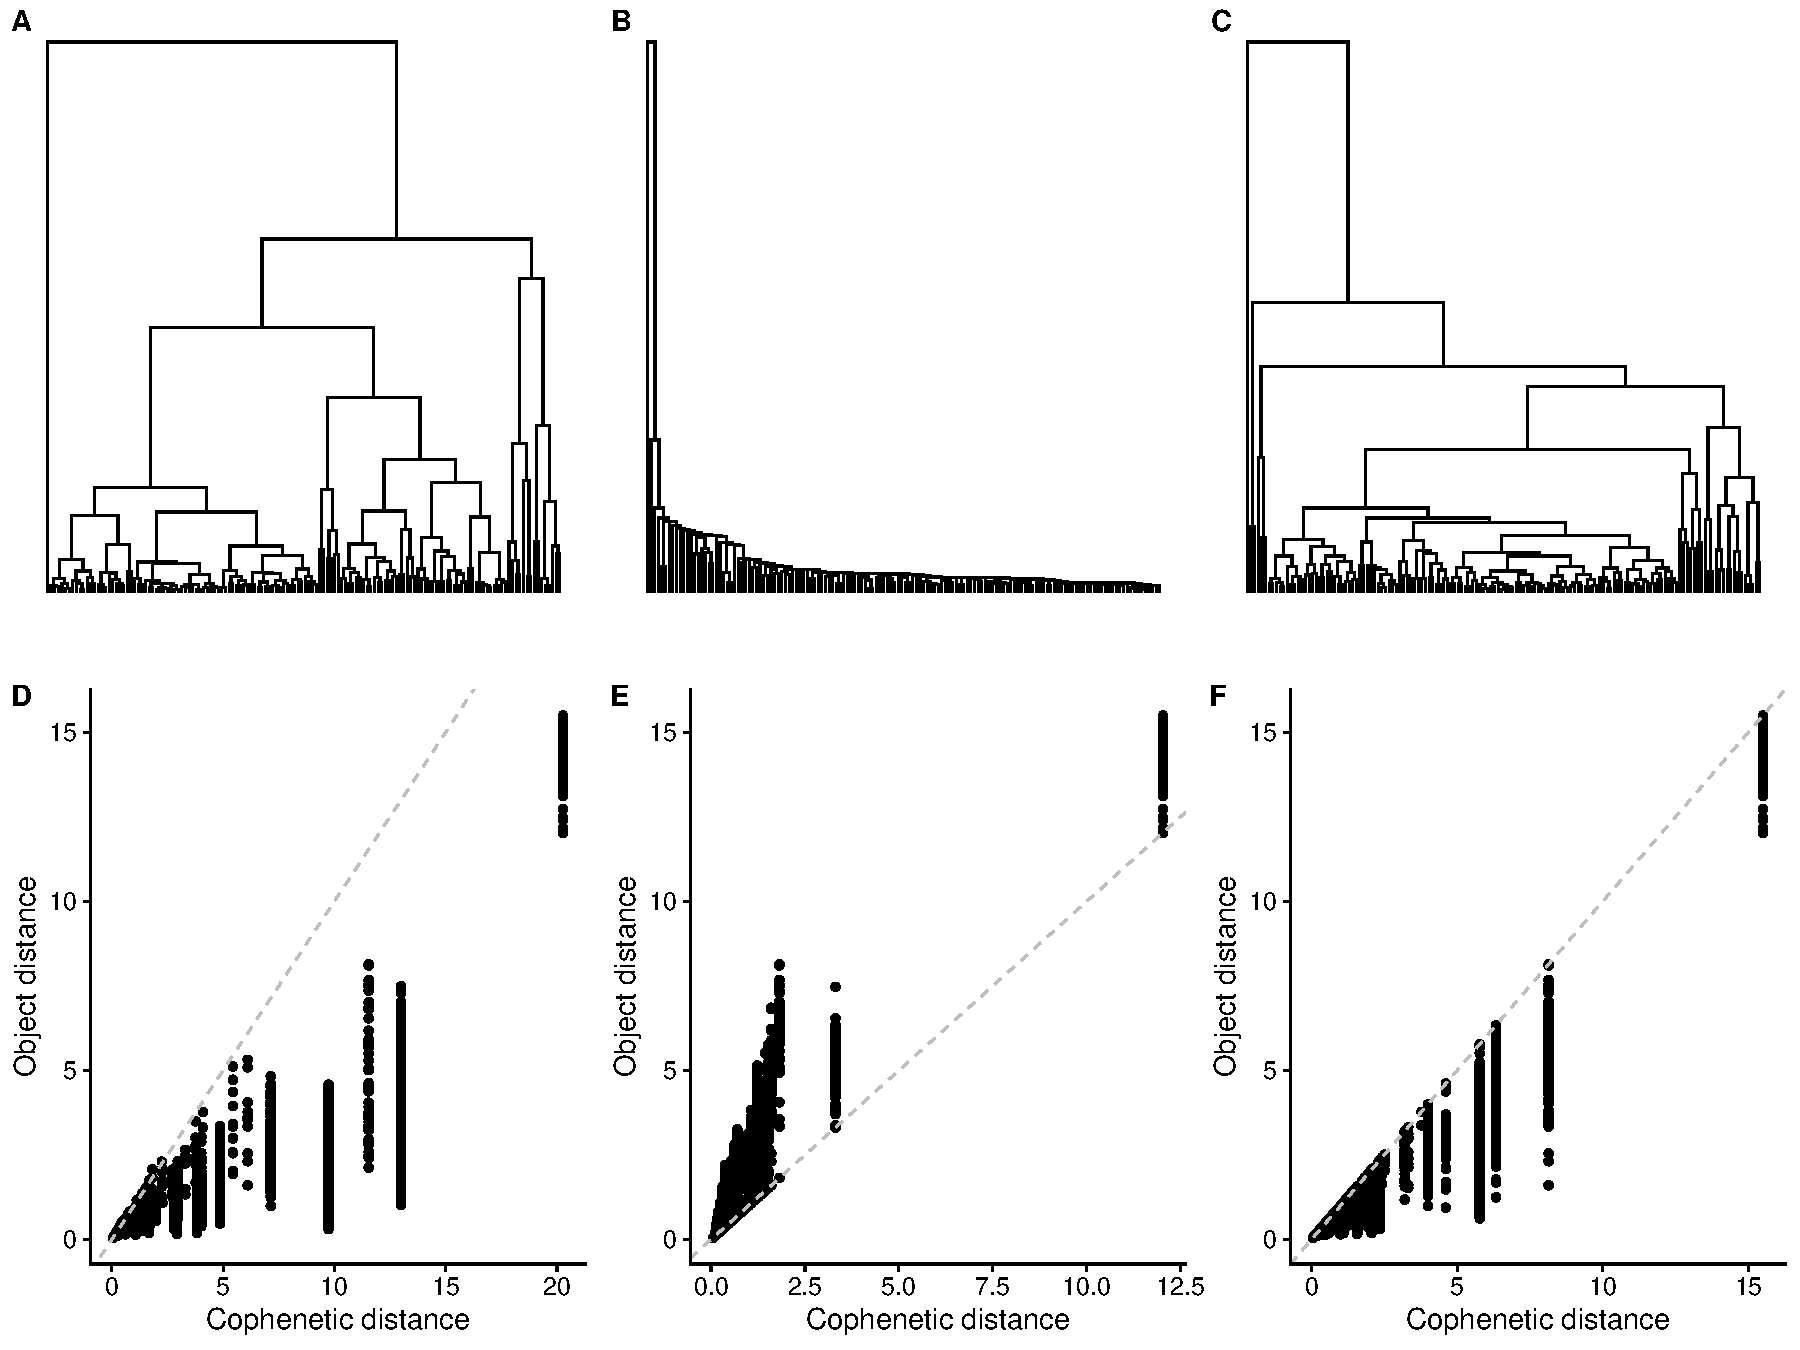
\includegraphics[width=\textwidth]{../figures/si-hc-plots-1} 

}

\caption{Plots for the hierarchical cluster analysis of the movement summary indicators computed for 142 Mongolian nomadic households with at least 3 campsite locations using three different clustering algorithms (Ward's minimum variance clustering (WMVC): left column, Single linkage clustering (SLC): middle column, Complete linkage clustering (CLC): right row). Upper row: Dendrograms. Lower row: Plots of the Euclidean distance between households based on their movement summary indicators in dependency of the cophenetic distances derived from the clustering results. The dashed line represents the case where the cophenetic distance and the Euclidean distance are identical.}\label{fig:si-hc-plots}
\end{figure}

\hypertarget{regression-analysis-1}{%
\subsection{Regression Analysis}\label{regression-analysis-1}}

According to the regression model, the total distance covered by a
household within the study period is positively related to both the
number of visited campsite locations (95 \%-confidence interval on the
link scale: {[}1.35; 1.82{]}) and the median distance between subsequent
campsite locations (95 \%-confidence interval on the link scale:
{[}1.94; 2.5{]}) (figure 6):

A household with four campsite locations, and a median distance between
subsequent campsite locations of 10 km (that covers a distance of 40 km
according to the model) that would visit one more campsite location
would increase its total distance covered on average by 17 km. If the
same household would increase the median distance between subsequent
campsite locations by 1 km, it would increase its total distance covered
on average by 3 km. The model underestimated the total distance covered
by one household that apparently made one or few movements over a large
distance since it visited both a non-extreme number of campsite
locations and had an extreme median distance between subsequent campsite
locations (figure 11). Overall, the model explained around 81 \% of the
variance.

A Scatterplot relating the total distance covered to the median distance
between subsequent campsite locations, and the number of visited
campsite locations reveals that these three movement indicators
interrelate gradually (figure 6). This gradient has three conceptual
extrema (figure 6): The first extremum are households that covered a
relatively small total distance, visited only few campsite locations and
had a relatively small distance between subsequent campsite locations.
The two other extrema are formed by two distinct groups of households
covering a total distance of approximately \(\ge170\) km, besides the
bulk of the sampled households covering total distances of approximately
\(<170\) km (figure 6): Households representing the second extremum have
a median distance between subsequent campsite locations corresponding
roughly to the average of the median distances between subsequent
campsite locations of the bulk of the sampled households (12 km), but
visited a relatively large number of campsite locations (6 to 14).
Households representing the third extremum visited a relatively small
number of campsite locations (3 to 6), but had a larger median of the
median distances between subsequent campsite locations than all
remaining households (36 km). For the bulk of the sampled households,
there exists a gradient in the total distance covered that can be
explained by both the number of visited campsite locations and the
median distance between subsequent campsite locations (figure 6).

\begin{figure}[H]

{\centering 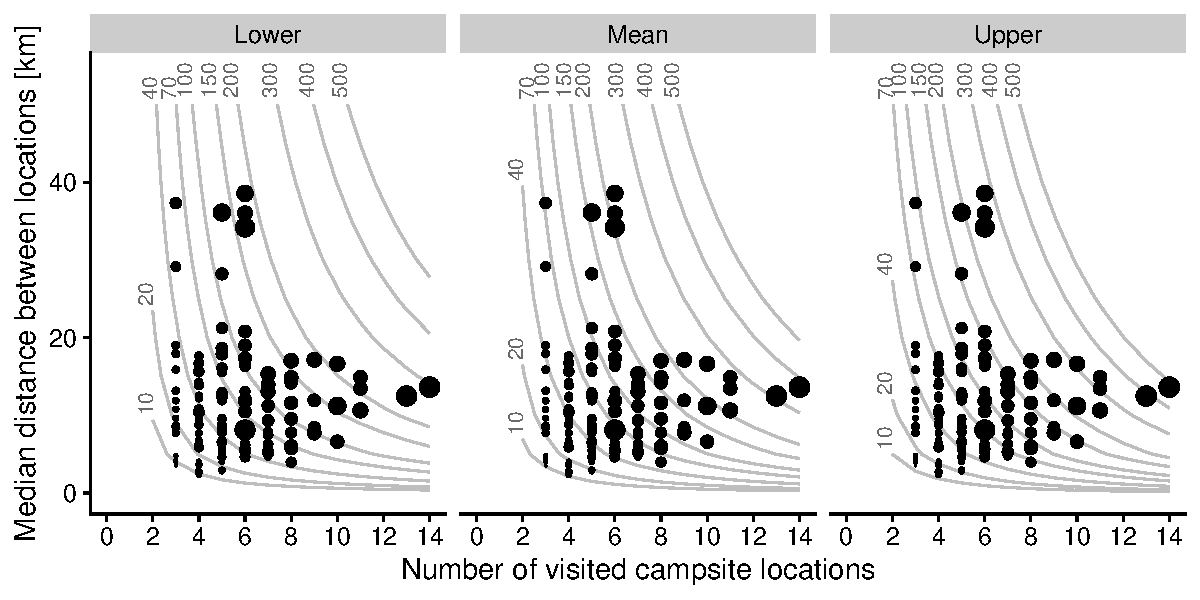
\includegraphics[width=\textwidth]{../figures/regression-plots1-1} 

}

\caption{Contour plot of the predicted values for the total distance covered in dependency of the number of visited campsite locations and the median distance between subsequent campsite locations [km]. The first and last column contain the lower and upper 95 \% confidence intervals, respectively, and the middle column the predicted mean value. Different lines and their labels indicate different levels of the predicted total distance [km]. Points represent non-modeled data points and are scaled relative to the unpredicted total distances covered. One extreme observation (median distance between subsequent locations: 126 km, number of locations: 3, total distance covered: 269 km) has been removed from the plot to facilitate visual differentiaion of the remaining observations.}\label{fig:regression-plots1}
\end{figure}

\hypertarget{discussion}{%
\section{Discussion}\label{discussion}}

\hypertarget{nomadic-movement-strategies}{%
\subsection{Nomadic Movement
Strategies}\label{nomadic-movement-strategies}}

\hypertarget{three-strategies-of-nomadic-movement}{%
\subsubsection{Three Strategies of Nomadic
Movement}\label{three-strategies-of-nomadic-movement}}

The main conclusion of the PCA and HCA concerning movement strategies of
households is that households gradually vary with respect to their
mobility range, i.e.~the total distance covered. The linear regression
analysis provided more insight into how different movement strategies
enable different households to increase their total distance covered.
Along this gradient, three extreme movement strategies can be
characterized (figure 6): First, there are households visiting few
campsite locations and having a low median distance between subsequent
campsite locations, and consequently a small total distance covered.
Second, there are households visiting a large number of campsite
locations, but having average median distances between subsequent
campsite locations. Third, there are households visiting an average
number of campsite locations, but having clearly above-average median
distances between subsequent campsite locations. These households more
frequently make long-distance movements between subsequent campsite
locations. It is important to note that our data suggests that
households vary gradually in how they adopt these movement strategies.
There exist no distinct clusters based only on these three strategies.

Whilst it is generally not surprising that households cover differing
distances and that the three described movement strategies exist, we
emphasize on the importance of quantitatively confirming these findings
and providing means of measuring a household's mobility range and its
movement strategy. \%, which is of great relevance for nomad's
livelihoods in general: Mobility is what differentiates nomads from
settled pastorals. Mobility guarantees access to a larger amount of
resources (water and forage) for the livestock and thus enables
households to possess larger herds and to better cope or adapt to
weather extremes (Fernández-Giménez et al., 2015).

Fernández-Giménez et al. (2015) identified mobility as one of the most
important factors for Mongolian herders to cope with extreme winter
conditions. The number of visited campsite locations is related to the
pasture area a household's herd can use. Hence, increasing the number of
visited campsite locations allows a household to use more resources than
a household with fewer pastures under the same environmental conditions.
Conversely, a household with a larger herd may have to move more
frequently in order to provide enough forage for the livestock.

The median distance between subsequent campsite locations does not only
denote a kind of average distance covered during individual movements,
but also comprises information on the relative frequency of movements of
this distance per household. Households with a larger median distance
between subsequent campsite locations typically cover distances of at
least this distance, i.e.~in approximately 50 \% of the individual
movements. Typically larger distances per individual movement may be a
consequence of missing access to nearby pastures (e.g.~because of other
herders having a campsite location in this area, or because of
unfavorable pasture conditions) or socioeconomic reasons (see below).
The first case expresses a strategy to increase resource use in contrast
to not moving or moving to pastures with less resources available.

Marin (2008) points out the importance of the costs of moving.
Movement-related issues (long distances to cover, petrol prices) were
considered as very important by interviewed herders (Marin, 2008).
Households covering larger total distances have to spend more resources
on movement than households covering smaller total distances.

Synthesized, this shows that mobility is fundamental for Mongolian
nomadic households to sustain their livelihood, by resulting in a
trade-off between both access to resources and transportation costs, and
to be able to cope with weather extremes. Different movement strategies
are likely to result in different resource use efficiencies under
different environmental (e.g.~forage availability in dependency of the
landscape type) and socioeconomic (e.g.~access to means of transport)
conditions.

Our findings show that GPS-based studies represent a framework to
capture and quantitatively measure these different movement strategies
of nomadic herders. Such a framework is needed for a deeper
understanding of how nomadic movement relates to environmental and
socioeconomic conditions.

\hypertarget{comparison-to-qualitative-studies}{%
\subsection{Comparison to Qualitative
Studies}\label{comparison-to-qualitative-studies}}

\hypertarget{reported-ranges-for-the-total-distance-covered-and-the-number-of-visited-campsite-locations}{%
\subsubsection{Reported ranges for the total distance covered and the
number of visited campsite
locations}\label{reported-ranges-for-the-total-distance-covered-and-the-number-of-visited-campsite-locations}}

Any comparisons with existing studies on Mongolian nomadic movement must
be treated cautiously: First, existing studies use qualitative methods
and detailed information on data collection (e.g.~sample sizes) are
often not available. Second, most existing studies were conducted prior
1990, the year Mongolia became a democracy and free-market economy
(Fernández-Giménez et al., 2015). Afterwards, movement patterns, such as
the total distance covered, most likely changed due to a privatization
of the herding economy and increased access to means of transportation
(Fernández-Giménez, 2006, p. @Marin.2008). Jagvaral (1975) and Batnasan
(1978) reported on movement patterns of Mongolian nomads during the
Soviet time. We found only one study reporting on Mongolian herders'
movement patterns based on data collected after 1990 (Ganbold, 2015).
Third, since movement patterns are heterogeneous and extreme values of
certain movement summary indicators have a low density, studies with low
sample sizes are likely to miss extreme values. Consequently it is not
possible to attribute differences to either societal, technological or
sampling issues. Nevertheless, it is important for future research to
set our data in the context of existing studies.

The ranges of the mobility range roughly agree with the values reported
qualitatively in previous studies (Jagvaral, 1975, pp. @Batnasan.1978,
@Ganbold.2015). However, there are also some differences: 8 and 4 out of
the 142 analyzed households had a total distance covered \(>200\) km and
\(>300\) km, respectively, in contrast to the upper bounds of 100, 200
and 300 km given by Jagvaral (1975), Ganbold (2015) and Batnasan (1978),
respectively. Jagvaral (1975) found that some households had up to 20
campsite locations, whereas we detected with our approach at maximum 14
campsite locations. Any household with \(\ge10\) campsite locations in
the sample covered at least 139 km, in contrast to the 50 to 100 km
reported by Jagvaral (1975). Ganbold (2015) reported movement ranges of
40 to 200 km and 4 to 8 visited campsite locations. Thus, the range of
total distances covered reported by Ganbold (2015) is narrower than the
values we found. The same is true for the number of campsite locations.

Given that we ensured a high quality of the analyzed data via
conservative gap filling and data filtering and that we certainly
underestimated the actual distance covered during movement (by
discarding short term visits and measuring only beeline distance), we
assume two possible reasons for this. Either Mongolian herders nowadays
cover larger distances in comparison to Soviet times (e.g.~because more
households move by truck or car instead of walking), or the qualitative
studies underestimated the distance covered.

\hypertarget{categorizing-households-based-on-movement-characteristics}{%
\subsubsection{Categorizing households based on movement
characteristics}\label{categorizing-households-based-on-movement-characteristics}}

Qualitative studies often tried to categorize the mobility range and
number of campsite locations based on distinct movement characteristics,
geographical regions or landscape types (Simukov, 1934, pp.
@Tsevel.1934, @Jagvaral.1975, @Batnasan.1978, @Ganbold.2015). Our
analyses could not confirm the presence of distinct clusters based
solely on movement summary indicators, but instead indicate gradual
variations between the three identified extreme movement strategies.
This is in contrast to (Batnasan, 1978) who proposed a classification as
short distance or long distance movement, based on the total distance
covered. While we did not analyze the relation of movement patterns to
different land cover types or geographic regions, we argue that
classifications of movement patterns according to geographic regions or
landcover type are only a first attempt to understand the movement of
nomadic households.

Instead, we suggest that GPS based studies of trajectories make it
possible to directly analyze the relation between movement
characteristics and movement strategies on the one side and
environmental and socioeconomic conditions on the other side as
gradients. Such an approach has the potential to: (1) yield deeper
insights into how environmental conditions and socioeconomic data shape
nomadic household trajectories (for example how local long-term patterns
in snow depth affect the selection of campsite locations), (2) yield
deeper insights into if and how households with different movement
strategies cope/adapt differently with/to extreme weather events, such
as dzuds and (3) investigate how changes in climate conditions and
socioeconomic conditions may affect the livelihood of nomadic households
(e.g.~changes in future forage availability). To summarize, we suggest
that GPS-based studies on nomadic movement have the potential to give
new insights into socioeconomic relevant mechanisms if intersected with
environmental and socioeconomic data.

\hypertarget{gps-data-quality-and-drawbacks-of-the-presented-gps-based-approach}{%
\subsection{GPS Data Quality and Drawbacks of the Presented GPS-Based
Approach}\label{gps-data-quality-and-drawbacks-of-the-presented-gps-based-approach}}

During this study, the GPS loggers were attached to the main pole of the
ger of the herders. An observation made by the field team when
recollecting GPS loggers at the end of the study period was that they
were often switched off or ran out of power during movement. This
affects the data analysis in two ways. First, only beeline distances
between campsite locations could be measured, but the actual trajectory
in-between campsite locations is unknown. Second, exact dates of
arrivals and departures are unknown because information on when GPS
loggers were switched off or ran out of power and were again switched on
are not available. Apart from this, the data give reliable information
on the position of a household on almost daily basis, enabling to
quantitatively study nomadic movement with high temporal resolution. In
particular, scatterplots of the values of the computed movement summary
indicators in dependency of the proportion of gaps in the trajectory
data after preprocessing and filtering (figure 9) did not show clear
patterns or trends, indicating that the data are unbiased after
preprocessing and filtering. This shows that the approach is likely
suitable to generate unbiased information on nomadic movements.

Despite these promising results, it is important to note that only
around 37 \% of the expected data (147 out of 400 initial households)
could be used during our analysis. GPS loggers could not be retrieved or
did not contain any data for 13 \% (52) of the households and about half
of the households (201) for which data could be retrieved did not
fulfill our thresholds of at most 30 \% of gaps and no gap with a
duration longer than 30 days. We therefore recommend that future studies
should expect a data loss of approximately two thirds if GPS data are
recorded over a period of nearly one year and if a similar study period
length is targeted. For analyses targeting shorter time periods data
losses may be slightly lower.

\hypertarget{conclusions}{%
\section{Conclusions}\label{conclusions}}

Our findings show that studies using movement summary indicators derived
from GPS data present a suitable framework to quantitatively analyze
different mobility strategies of nomadic herders. With respect to the
movement of Mongolian herders, the results of the quantitative analysis
imply that: While there is a clear gradient in the mobility range of the
sampled households, it is difficult to categorize them into groups
characterized by distinct movement summary indicators alone. Instead,
there exists a continuous field of movement strategies with respect to
mobility range and the three extreme movement strategies described in
this study. Potential reasons for this are that movement strategies may
be highly adapted to environmental and socioeconomic conditions
individual households face. A combined analysis using additional data
describing these conditions as well as the movement summary indicators
proposed in this study may provide new insights into the adaption
strategies of Mongolian households and allow for assumptions on how they
will be impacted by changing climate conditions.

\hypertarget{acknowledgements}{%
\section{Acknowledgements}\label{acknowledgements}}

The research and data on which this study is based were generously
funded by Volkswagen Stiftung, funding initiative ``Between Europe and
the Orient'', research grant 88498. Kati Kraehnert was affiliated with
the German Institute for Economic Research while major parts of the
research presented here were conducted. Myagmartseren Purevtseren and
Munkhnaran Sugar were supported in 2019-2020 by the Asia Research
Center, National University of Mongolia - Korea Foundation for Advanced
Studies (ARC-KFAS), project number P2019-3743.

\hypertarget{references}{%
\section*{References}\label{references}}
\addcontentsline{toc}{section}{References}

\hypertarget{refs}{}
\begin{cslreferences}
\leavevmode\hypertarget{ref-Barton.2020}{}%
Barton, K., 2020. MuMIn: Multi-Model Inference.

\leavevmode\hypertarget{ref-Batnasan.1978}{}%
Batnasan, G., 1978. The Method of Managing the Collective Farming of the
People's Republic of Mongolia, 6th ed. Ulaanbaatar.

\leavevmode\hypertarget{ref-Borcard.2011}{}%
Borcard, D., Gillet, F., Legendre, P., 2011. Numerical Ecology with R.
Springer New York, New York, NY.
doi:\href{https://doi.org/10.1007/978-1-4419-7976-6}{10.1007/978-1-4419-7976-6}

\leavevmode\hypertarget{ref-FernandezGimenez.2006}{}%
Fernández-Giménez, M.E., 2006. Land Use and Land Tenure in Mongolia: a
Brief History and Current Issues. USDA Forest Service Proceedings.

\leavevmode\hypertarget{ref-FernandezGimenez.2018}{}%
Fernández-Giménez, M.E., Allington, G.R.H., Angerer, J., Reid, R.S.,
Jamsranjav, C., Ulambayar, T., Hondula, K., Baival, B., Batjav, B.,
Altanzul, T., Baasandorj, Y., 2018. Using an Integrated
Social-Ecological Analysis to Detect Effects of Household Herding
Practices on Indicators of Rangeland Resilience in Mongolia.
Environmental Research Letters 13, 075010.
doi:\href{https://doi.org/10.1088/1748-9326/aacf6f}{10.1088/1748-9326/aacf6f}

\leavevmode\hypertarget{ref-FernandezGimenez.1996}{}%
Fernández-Giménez, M.E., Batbuyan, B., Oyungerel, J., 1996.
Socio-Economic Aspects of the Pastoral Movement Patterns of Mongolian
Herders, in: Humphrey, C., Sneath, D. (Eds.), Culture and Environment in
Inner Asia Volume 1. The Pastoral Economy and the Environment. White
Horse Press, Cambridge, pp. 58--110.

\leavevmode\hypertarget{ref-FernandezGimenez.2007}{}%
Fernández-Giménez, M.E., Batbuyan, B., Oyungerel, J., 2007. Climate,
Economy and Land Policy: Effects on Pastoral Mobility Patterns in
Mongolia, in: Sun, X., Naito, N. (Eds.), Mobility, Flexibility, and
Potential of Nomadic Pastoralism in Eurasia and East Africa. Kyoto
University, Kyoto, pp. 3--24.

\leavevmode\hypertarget{ref-FernandezGimenez.2015}{}%
Fernández-Giménez, M.E., Batkhishig, B., Batbuyan, B., Ulambayar, T.,
2015. Lessons from the Dzud: Community-Based Rangeland Management
Increases the Adaptive Capacity of Mongolian Herders to Winter
Disasters. World Development 68, 48--65.
doi:\href{https://doi.org/10.1016/j.worlddev.2014.11.015}{10.1016/j.worlddev.2014.11.015}

\leavevmode\hypertarget{ref-Galili.2015}{}%
Galili, T., 2015. dendextend: an R Package for Visualizing, Adjusting
and Comparing trees of Hierarchical Clustering. Bioinformatics (Oxford,
England) 31, 3718--3720.
doi:\href{https://doi.org/10.1093/bioinformatics/btv428}{10.1093/bioinformatics/btv428}

\leavevmode\hypertarget{ref-Ganbold.2015}{}%
Ganbold, N., 2015. Traditions and Modern Trends of Mongolian Herders'
Movement.

\leavevmode\hypertarget{ref-Hahsler.2019}{}%
Hahsler, M., Piekenbrock, M., 2019. dbscan: Fast Density-Based
Clustering with R.

\leavevmode\hypertarget{ref-Himmelsbach.2012}{}%
Himmelsbach, R., 2012. Collaborative Pasture Management: A Solution for
Grassland Degradation in Mongolia?, in: Dierkes, J.B. (Ed.), Change in
democratic Mongolia, Brill's Inner Asian library. Brill, Leiden, pp.
165--195.

\leavevmode\hypertarget{ref-Hocking.2020}{}%
Hocking, T.D., 2020. directlabels: Direct Labels for Multicolor Plots.

\leavevmode\hypertarget{ref-IntergovernmentalPanelonClimateChange.2007}{}%
Intergovernmental Panel on Climate Change, 2007. Climate Change 2007:
Synthesis Report of the Fourth Assessment Report. Geneva.

\leavevmode\hypertarget{ref-IntergovernmentalPanelonClimateChange.2013}{}%
Intergovernmental Panel on Climate Change, 2013. Climate Change 2013:
The Physical Science Basis. Geneva.

\leavevmode\hypertarget{ref-IPCC.2014}{}%
Intergovernmental Panel on Climate Change, 2014. Climate Change 2014:
Impacts, Adaptation, and Vulnerability. Part A: Global and Sectoral
Aspects. Contribution of Working Group II to the Fifth Assessment Report
of the Intergovernmental Panel on Climate Change. Cambridge University
Press, Cambridge, United Kingdom; New York, NY, USA.

\leavevmode\hypertarget{ref-Jackson.1993}{}%
Jackson, D.A., 1993. Stopping Rules in Principal Components Analysis: A
Comparison of Heuristical and Statistical Approaches. Ecology 74,
2204--2214. doi:\href{https://doi.org/10.2307/1939574}{10.2307/1939574}

\leavevmode\hypertarget{ref-Jagvaral.1975}{}%
Jagvaral, N., 1975. The Issue of the Livestock Management System in the
People's Republic of Mongolia. Journal of Academy of Sciences.

\leavevmode\hypertarget{ref-Laube.2007}{}%
Laube, P., Dennis, T., Forer, P., Walker, M., 2007. Movement Beyond the
Snapshot -- Dynamic Analysis of Geospatial Lifelines. Computers,
Environment and Urban Systems 31, 481--501.
doi:\href{https://doi.org/10.1016/j.compenvurbsys.2007.08.002}{10.1016/j.compenvurbsys.2007.08.002}

\leavevmode\hypertarget{ref-LehmannUschner.2018}{}%
Lehmann-Uschner, K., Kraehnert, K., 2018. When Shocks Become Persistent:
Household-Level Asset Growth in the Aftermath of an Extreme Weather
Event. DIW Discussion Paper.
doi:\href{https://doi.org/10.1016/j.geoforum.2010.05.006}{10.1016/j.geoforum.2010.05.006}

\leavevmode\hypertarget{ref-Maechler.2018}{}%
Maechler, M., Rousseeuw, P., Struyf, A., Hubert, M., Hornik, K., 2018.
cluster: Cluster Analysis Basics and Extensions.

\leavevmode\hypertarget{ref-Marin.2008}{}%
Marin, A., 2008. Between Cash Cows and Golden Calves: Adaptations of
Mongolian Pastoralism in the 'Age of the Market'. Nomadic Peoples 12,
75--101.
doi:\href{https://doi.org/10.3167/np.2008.120206}{10.3167/np.2008.120206}

\leavevmode\hypertarget{ref-Murphy.2011}{}%
Murphy, D., 2011. Going on Otor: Disaster, Mobility, and the Political
Ecology of Vulnerability in Uguumur, Mongolia (PhD thesis). University
of Kentucky; Anthropology, University of Kentucky, Lexington.

\leavevmode\hypertarget{ref-Nakagawa.2017}{}%
Nakagawa, S., Johnson, P.C.D., Schielzeth, H., 2017. The coefficient of
determination R2 and intra-class correlation coefficient from
generalized linear mixed-effects models revisited and expanded. Journal
of the Royal Society, Interface 14.
doi:\href{https://doi.org/10.1098/rsif.2017.0213}{10.1098/rsif.2017.0213}

\leavevmode\hypertarget{ref-NationalStatisticsOfficeofMongolia.2019}{}%
National Statistics Office of Mongolia, 2019. Mongolian Statistical
Information Service.

\leavevmode\hypertarget{ref-Oksanen.2018}{}%
Oksanen, J., Blanchet, F.G., Friendly, M., Kindt, R., Legendre, P.,
McGlinn, D., Minchin, P.R., O'Hara, R.B., Simpson, G.L., Solymos, P.,
Stevens, M.H.H., Szoecs, E., Wagner, H., 2018. vegan: Community Ecology
Package.

\leavevmode\hypertarget{ref-Pebesma.2018}{}%
Pebesma, E., Klus, B., Moradi, M., 2018. trajectories: Classes and
Methods for Trajectory Data.

\leavevmode\hypertarget{ref-RCoreTeam.2017}{}%
R Core Team, 2017. R: A Language and Environment for Statistical
Computing.

\leavevmode\hypertarget{ref-Sankey.2012}{}%
Sankey, T.T., Sankey, J., Weber, K., Montagne, C., 2012. Changes in
Pastoral Land Use and Their Effects on Rangeland Vegetation Indices, in:
Dierkes, J.B. (Ed.), Change in democratic Mongolia, Brill's Inner Asian
library. Brill, Leiden, pp. 149--163.
doi:\href{https://doi.org/10.1163/9789004231474_009}{10.1163/9789004231474\_009}

\leavevmode\hypertarget{ref-Seneviratne.2012}{}%
Seneviratne, S.I., Neville Nicholls, David Easterling, Goodess, C.M.,
Shinjiro Kanae, James Kossin, Yali Luo, Jose Marengo, Mc Innes, K.,
Mohammad Rahimi, Markus Reichstein, Asgeir Sorteberg, Carolina Vera,
Xuebin Zhang, Matilde Rusticucci, Vladimir Semenov, Alexander, L.V.,
Simon Allen, Gerardo Benito, Cavazos Perez, M.T., John Clague, Declan
Conway, Della-Marta, P.M., Markus Gerber, Sunling Gong, Goswami, B.N.,
Mark Hemer, Christian Huggel, van den Hurk, B., Kharin, V.V., Akio
Kitoh, Klein Tank, A.M.G., Guilong Li, Simon Mason, Mc Guire, W., van
Oldenborgh, G.J., Boris Orlowsky, Sharon Smith, Wassila Thiaw, Adonis
Velegrakis, Pascal Yiou, Tingjun Zhang, Tianjun Zhou, Zwiers, F.W.,
2012. Changes in Climate Extremes and their Impacts on the Natural
Physical Environment, in: Field, C.B., Barros, V., Stocker, T.F., Dahe,
Q. (Eds.), Managing the Risks of Extreme Events and Disasters to Advance
Climate Change Adaptation. Cambridge University Press, New York, pp.
109--230.
doi:\href{https://doi.org/10.1017/CBO9781139177245.006}{10.1017/CBO9781139177245.006}

\leavevmode\hypertarget{ref-Simukov.1934}{}%
Simukov, A.D., 1934. Mongolian Herders. Ulaanbaatar.

\leavevmode\hypertarget{ref-Stern.2011}{}%
Stern, N.H., 2011. The Economics of Climate Change: The Stern Review, 1.
ed., 7. print. ed. Cambridge Univ. Press, Cambridge.

\leavevmode\hypertarget{ref-Sternberg.2010}{}%
Sternberg, T., 2010. Unravelling Mongolia's Extreme Winter Disaster of
2010. Nomadic Peoples 14, 72--86.

\leavevmode\hypertarget{ref-Teickner.2020}{}%
Teickner, H., Knoth, C., 2020. herdersTA: Extracting Movement
Characteristics from GPS Trajectories of Nomadic Households.

\leavevmode\hypertarget{ref-Tsevel.1934}{}%
Tsevel, Y., 1934. Herders. Modern Mongolia.

\leavevmode\hypertarget{ref-Upton.2005}{}%
Upton, C., 2005. Institutions in a Pastoral Society: Processes of
Formation and Transformation in Postsocialist Mongolia. Comparative
Studies of South Asia, Africa and the Middle East 25, 584--559.

\leavevmode\hypertarget{ref-Upton.2010}{}%
Upton, C., 2010. Living off the Land: Nature and Nomadism in Mongolia.
Geoforum 865--874.
doi:\href{https://doi.org/10.1016/j.geoforum.2010.05.006}{10.1016/j.geoforum.2010.05.006}

\leavevmode\hypertarget{ref-Venables.2007}{}%
Venables, W.N., Ripley, B.D., 2007. Modern applied statistics with S, 4.
ed., corr. print. ed, Statistics and computing. Springer, New York, NY.

\leavevmode\hypertarget{ref-Wickham.2016}{}%
Wickham, H., 2016. ggplot2: Elegant Graphics for Data Analysis, Use R!
Springer, Cham.
doi:\href{https://doi.org/10.1007/978-3-319-24277-4}{10.1007/978-3-319-24277-4}

\leavevmode\hypertarget{ref-Wilke.2018}{}%
Wilke, C.O., 2018. cowplot: Streamlined Plot Theme and Plot Annotations
for 'ggplot2'.

\leavevmode\hypertarget{ref-WorldBank.2009}{}%
World Bank, 2009. Mongolia: Livestock Sector Study. Washington, DC.
\end{cslreferences}

\clearpage

\appendix

\hypertarget{definition-of-movement-summary-indicators}{%
\section{Definition of Movement Summary
Indicators}\label{definition-of-movement-summary-indicators}}

\begin{figure}[H]

{\centering 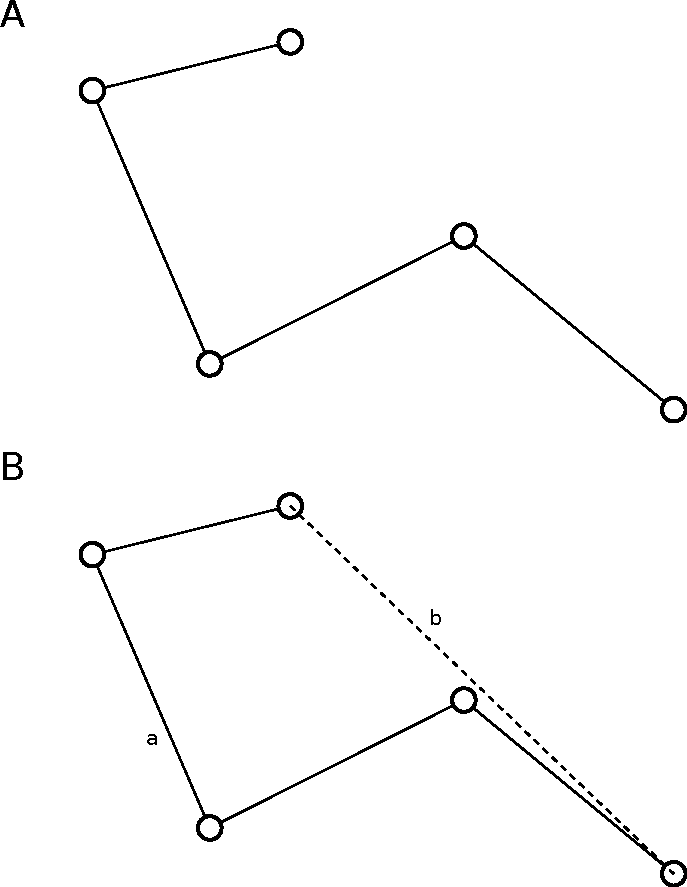
\includegraphics[width=0.65\textwidth]{./../figures/si_definition_straighntess_index} 

}

\caption{Conceptual representation of the definition of the straightness index Laube et al. 2007. Points represent campsite locations in each panel. A: A sample trajectory. B: The straightness index is computed by (1) drawing a line between the start and end point of the trajectory (dashed line) and (2) dividing the length of the trajectory ($a$) by the length of the line between the start and end point of the trajectory ($b$).}\label{fig:appendix-definition-straightness-index}
\end{figure}

\begin{figure}[H]

{\centering 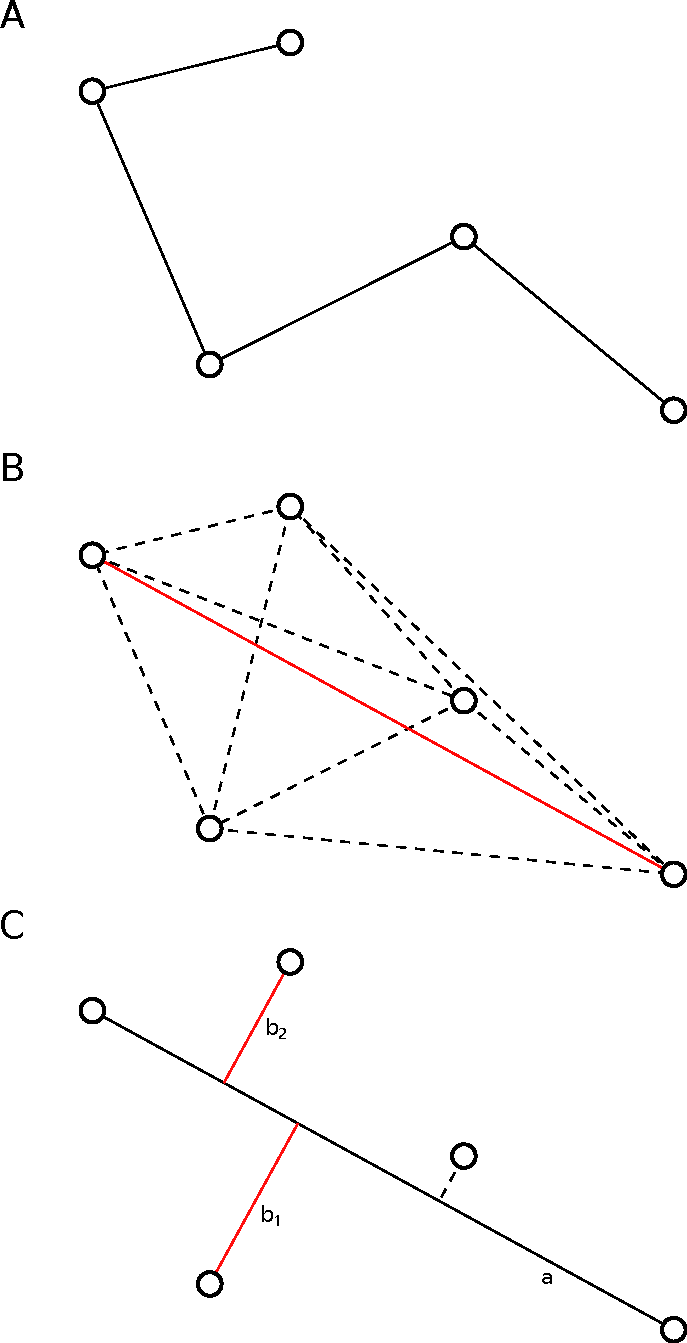
\includegraphics[width=0.65\textwidth]{./../figures/si_definition_linearity_tot} 

}

\caption{Conceptual representation of the definition of the linearity of a trajectory and how it is estimated. Points represent campsite locations in each panel. A: A sample trajectory. B: As first step, the pairwise distances between all campsite locations are computed (represented as dashed lines) and the maximum distance line (red) is kept and its length a is recorded. C: As second step, the shortest distances of all campsite locations to the kept line are computed and it is recorded for each campsite location, on which side of the line it is. If all campsite locations are on the same side of the line, the maximum distance is recorded and linearity is computed as the ratio of this distance and $a$. If there are campsite locations on both sides of the line, the maximum sum of two distances of campsite locations on different sides of the line are recorded ($b = b_1 + b_2$, red) and linearity is computed as $b/a$.}\label{fig:appendix-definition-linearity}
\end{figure}

\hypertarget{scatterplots-of-all-movement-summary-indicators-in-dependency-of-the-proportion-of-gaps-in-the-trajectory-data-after-preprocessing-and-filtering}{%
\section{Scatterplots of all Movement Summary Indicators in Dependency
of the Proportion of Gaps in the Trajectory Data after Preprocessing and
Filtering}\label{scatterplots-of-all-movement-summary-indicators-in-dependency-of-the-proportion-of-gaps-in-the-trajectory-data-after-preprocessing-and-filtering}}

\begin{figure}[H]

{\centering 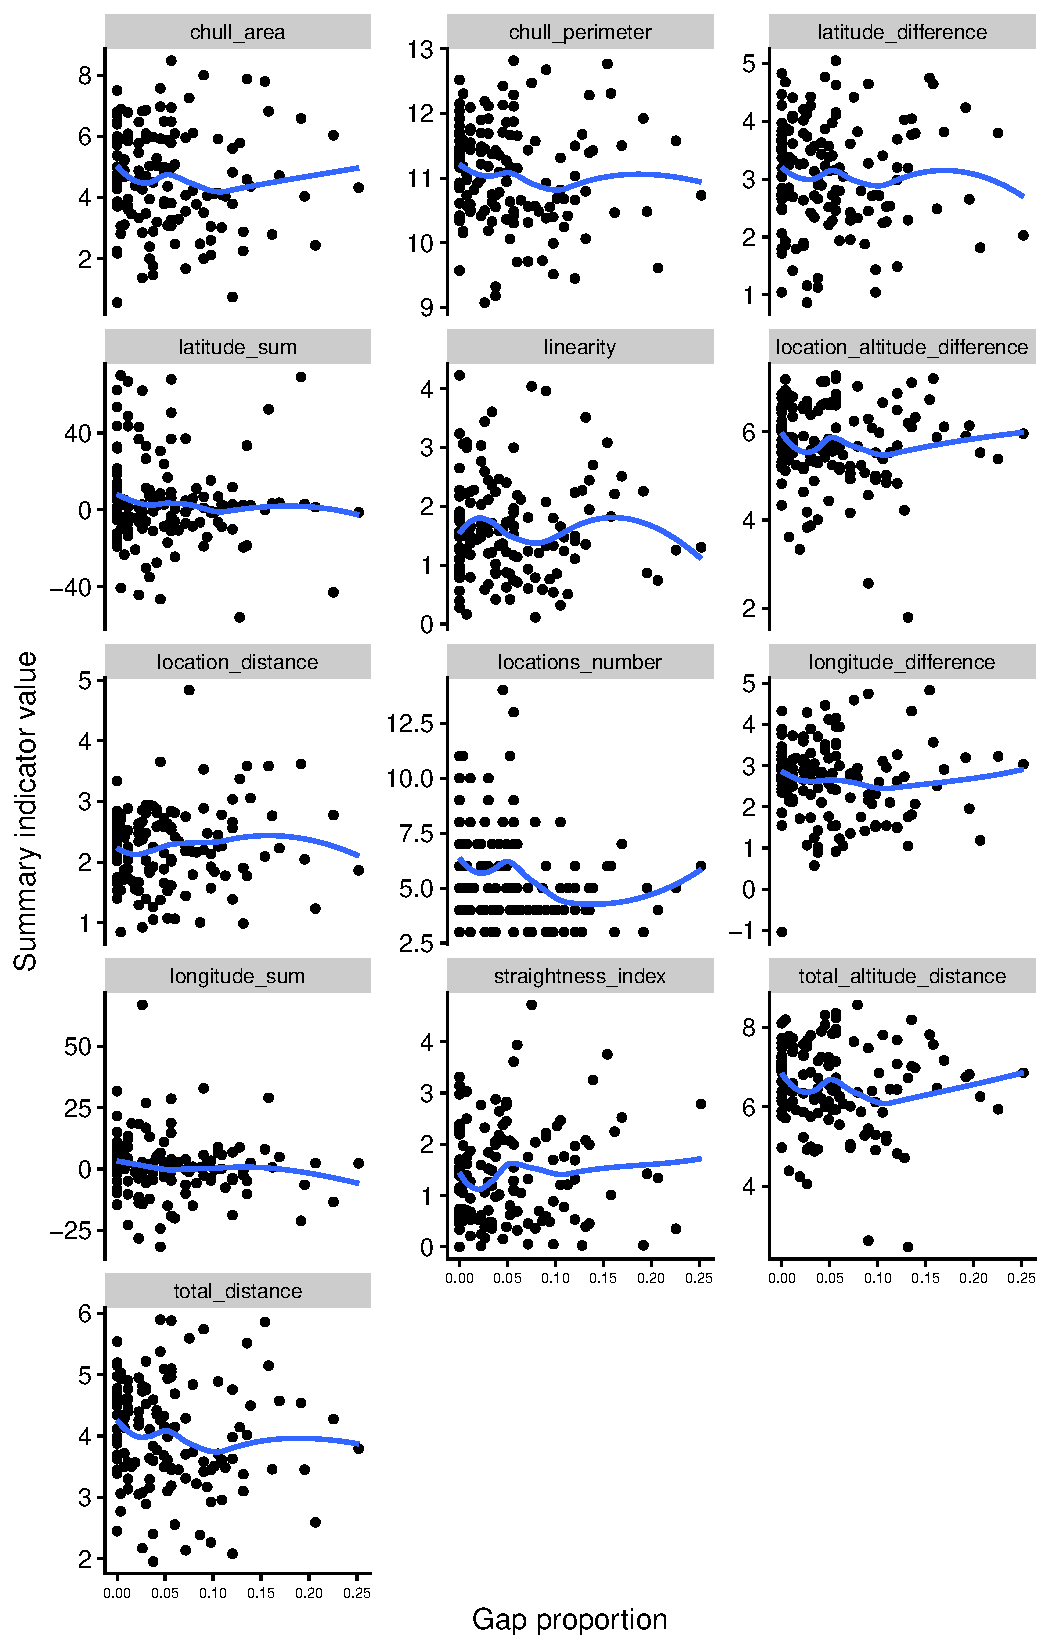
\includegraphics[width=0.75\textwidth]{../figures/appendix-si-gaps-plot-1} 

}

\caption{Scatterplots of the values of each summary indicator in dependency of the proportion of gaps in the trajectory data for each of the 142 households with a maximum proportion of missing values of 30 \% and a maximum duration of any gap of 30 days.}\label{fig:appendix-si-gaps-plot}
\end{figure}

\hypertarget{density-plots-of-skewed-movement-summary-indicator-variables-before-and-after-transformation}{%
\section{Density Plots of Skewed Movement Summary Indicator Variables
Before and After
Transformation}\label{density-plots-of-skewed-movement-summary-indicator-variables-before-and-after-transformation}}

\begin{figure}[H]

{\centering 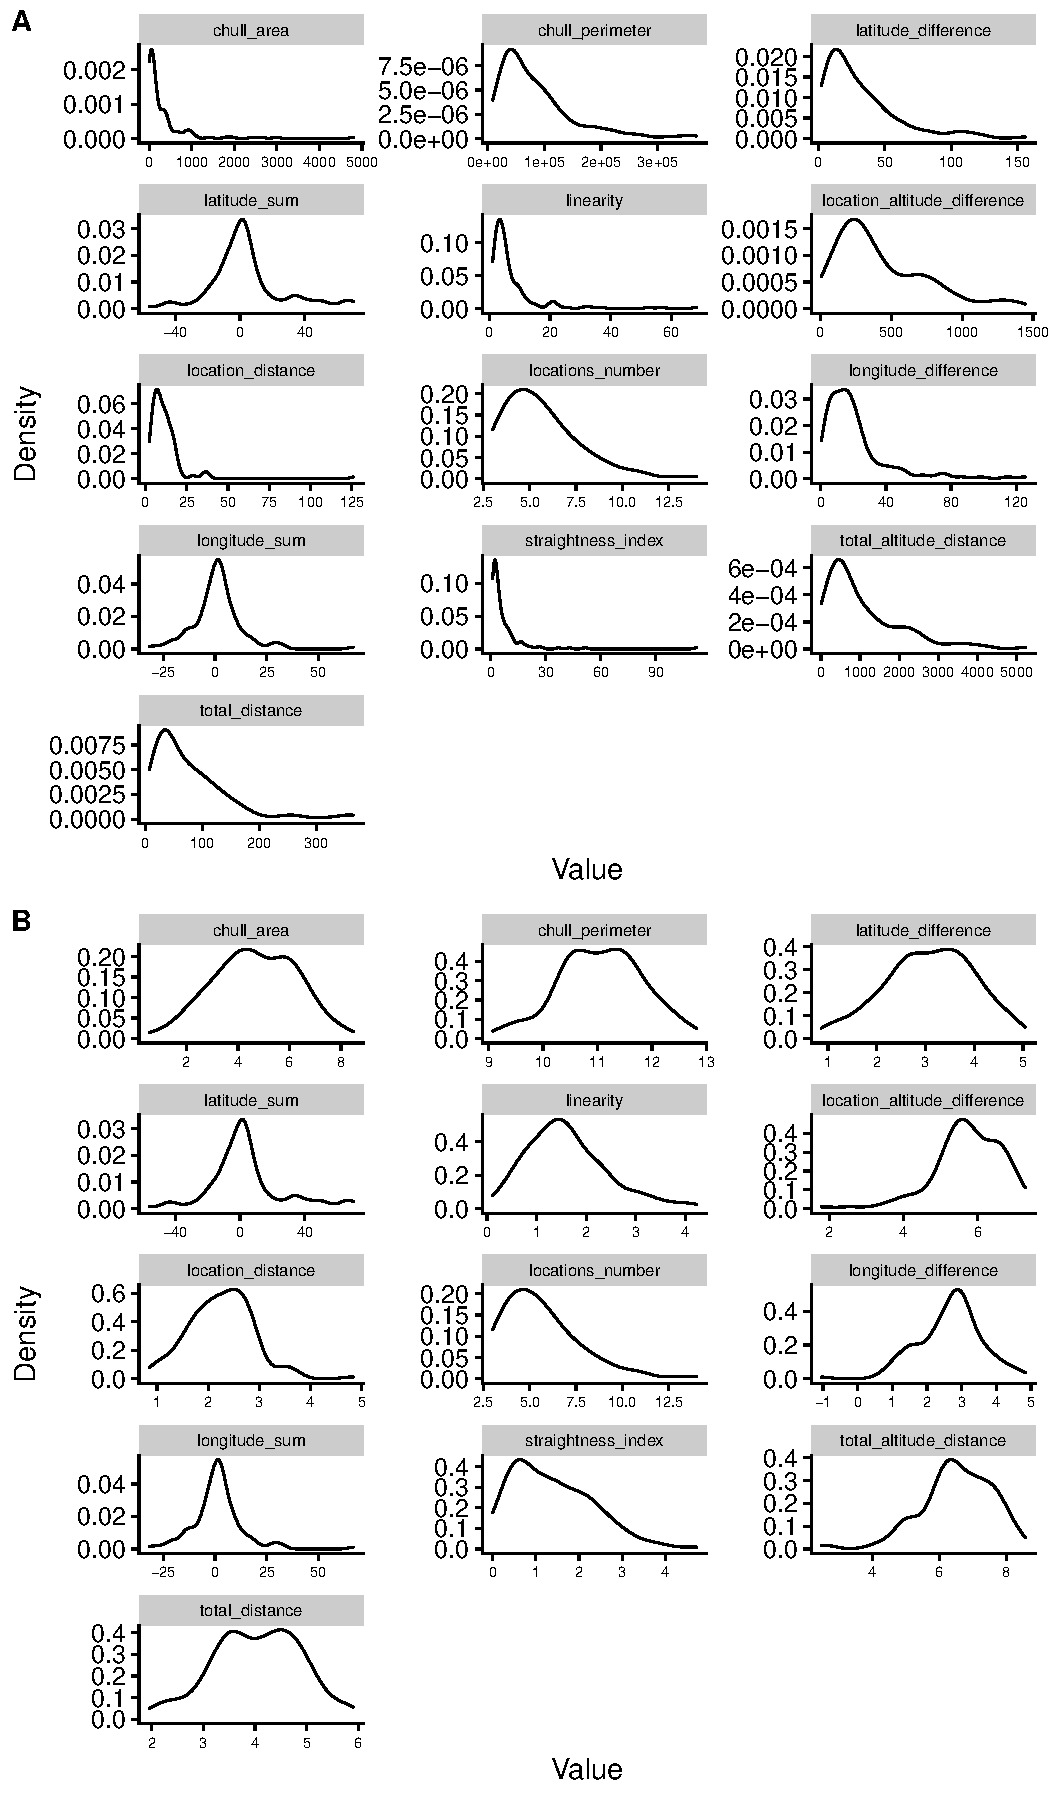
\includegraphics[width=0.75\textwidth]{../figures/appendix-si-density-plot-1} 

}

\caption{Density plots of movement summary indicator variables for the sampled Mongolian households with at least 3 campsite locations and skewed variables (chull\_area, chull\_perimeter, location\_altitude\_difference, location\_distance, longitude\_difference, latitude\_difference, straightness\_index, total\_altitude\_distance, total\_distance and linearity) before (A) and after (B) log transformation.}\label{fig:appendix-si-density-plot}
\end{figure}

\hypertarget{validation-plots-for-the-linear-regression-model}{%
\section{Validation Plots for the Linear Regression
Model}\label{validation-plots-for-the-linear-regression-model}}

\begin{figure}[H]

{\centering 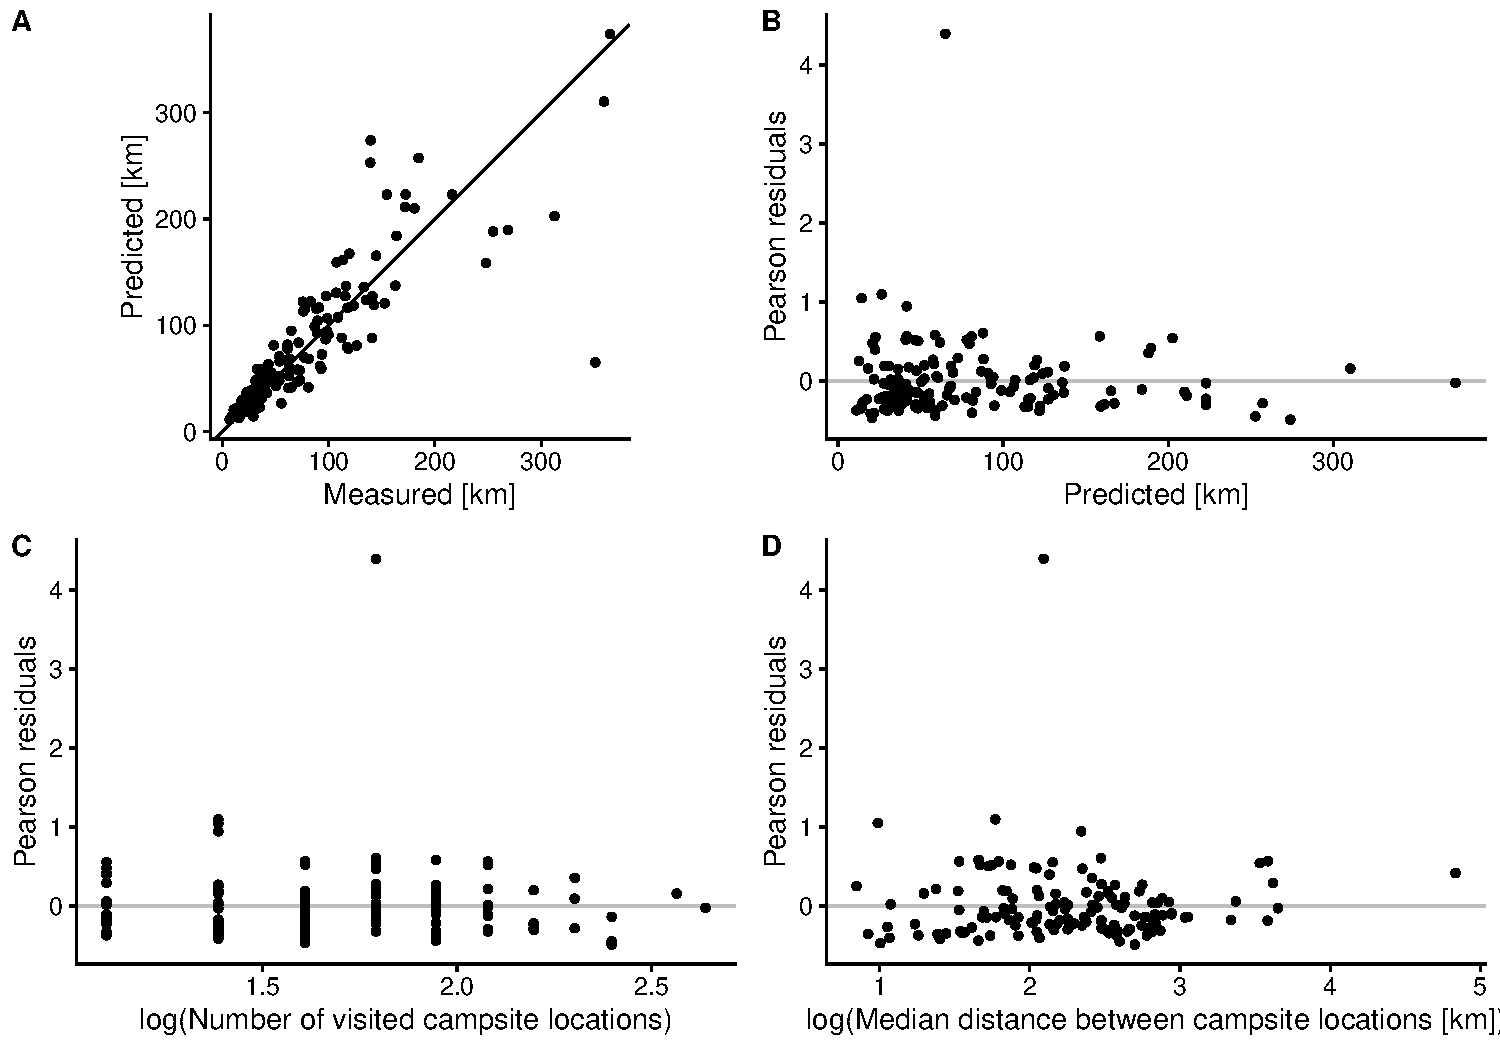
\includegraphics[width=0.8\textwidth]{../figures/regression-total-distance-validation-1} 

}

\caption{Validation plots for the regression model describing the total distance covered in dependency of the number of visited campsite locations and the median distance between subsequent campsite locations. A: Predicted values in dependency of measured values. Note that the axes are scaled equally. B: Residuals in dependency of predicted values. C: Residuals in dependency of the logarithmic number of visited campsite locations. D: Residuals in dependency of the logarithmic median distance between subsequent campsite locations.}\label{fig:regression-total-distance-validation}
\end{figure}


\end{document}

